\documentclass[12pt,letterpaper]{article}
\usepackage{inverba}
\newcommand{\userName}{Cullyn Newman} 
\newcommand{\class}{BI 213} 
\newcommand{\institution}{Portland State University} 
\newcommand{\thetitle}{\hypertarget{home}{Animals and Ecology}}
\rfoot{\hyperlink{home}{\thepage}}

\begin{document}

%%%%%%%%%%%%%%%%%%%%%%%%%%%%%%%%%%%%%%%%%%%%%%%%%%%%%%%%%%%%%%%%%%%%%%%%%%%%%%%%%%%%%%%%%
%                               %   %   %   %   %   %   %                               %
%                           %   %   %   %   %   %   %   %   %                           %
%                       %   %                               %   %                       %
%   %   %   %   %   %   %   %   O   U   T   L   I   N   E   %   %   %   %   %   %   %   %
%                       %   %                               %   %                       %
%                           %   %   %   %   %   %   %   %   %                           %
%                               %   %   %   %   %   %   %                               %
%%%%%%%%%%%%%%%%%%%%%%%%%%%%%%%%%%%%%%%%%%%%%%%%%%%%%%%%%%%%%%%%%%%%%%%%%%%%%%%%%%%%%%%%%
%\begingroup

\begin{contbox}{Animals and Ecology}{ 
\begin{enumerate}[font=\bfseries, wide]
    \setcounter{enumi}{38}
\item \hyperlink{39}{\textbf{Animal Form and Function}}
    \begin{itemize}
        \item \hyperlink{39.1}{Form, Function, and Adaptation}
        \item \hyperlink{39.2}{Tissues, Organs, and Systems}
        \item \hyperlink{39.3}{How Does Body Size Affect Animal Physiology?}
        \item \hyperlink{39.4}{Homeostasis}
        \item \hyperlink{39.5}{Thermoregulation: A Closer Look}
        \item \hyperlink{39.r}{Review}
    \end{itemize}
\item \hyperlink{40}{\textbf{Water and Electrolye Balance}}
    \begin{itemize}
        \item \hyperlink{40.1}{Osmoregulation and Exertion}
        \item \hyperlink{40.2}{Water and Electrolyte in Marine Fishes}
        \item \hyperlink{40.3}{Water and Electrolyte in Freshwater Fishes}
        \item \hyperlink{40.5}{Water and Electrolyte in Vertebrates}
        \item \hyperlink{40.r}{Review}
    \end{itemize}
\item \hyperlink{41}{\textbf{Nutrition}}
    \begin{itemize}
        \item \hyperlink{41.1}{Nutritional Requirements}
        \item \hyperlink{41.3}{How Are Nutrients Digested and Absorbed?}
        \item \hyperlink{41.4}{Nutritional Homeostasis}
        \item \hyperlink{41.r}{Review}
    \end{itemize}
\item \hyperlink{42}{\textbf{Gas Exchange}}
    \begin{itemize}
        \item \hyperlink{42.1}{The Resipitory and Circulatory System}
        \item \hyperlink{42.2}{Air and Water as Resipitory Media}
        \item \hyperlink{42.3}{Organs of Gas Exchange}
        \item \hyperlink{42.4}{How are Oxygen and Carbon Dioxide Transported in Blood?}
        \item \hyperlink{42.5}{Circulation}
        \item \hyperlink{42.r}{Review}
    \end{itemize}
\item \hyperlink{43}{\textbf{Nervous System}}
    \begin{itemize}
        \item \hyperlink{43.1}{Principles of Electric Signaling}
        \item \hyperlink{43.2}{Dissecting Action Potential}
        \item \hyperlink{43.3}{The Synapse}
        \item \hyperlink{43.4}{The Vertebrate Nervous System}
        \item [--] \hyperlink{43.r}{Review}
    \end{itemize}
\item \hyperlink{44}{\textbf{Sensory Systems}}
    \begin{itemize}
        \item 
    \end{itemize}
\item \hyperlink{45}{\textbf{Animal Movement}}
    \begin{itemize}
        \item 
    \end{itemize}
\item \hyperlink{46}{\textbf{Chemical Signals}}
    \begin{itemize}
        \item 
    \end{itemize}
\end{enumerate}
}\end{contbox}

%\endgroup
%%%%%%%%%%%%%%%%%%%%%%%%%%%%%%%%%%%%%%%%%%%%%%%%%%%%%%%%%%%%%%%%%%%%%%%%%%%%%%%%%%%%%%%%%
%                               %   %   %   %   %   %   %                               %
%                           %   %   %   %   %   %   %   %   %                           %
%                       %   %                               %   %                       %
%   %   %   %   %   %   %   %       N   O   T   E   S       %   %   %   %   %   %   %   %
%                       %   %                               %   %                       %
%                           %   %   %   %   %   %   %   %   %                           %
%                               %   %   %   %   %   %   %                               %
%%%%%%%%%%%%%%%%%%%%%%%%%%%%%%%%%%%%%%%%%%%%%%%%%%%%%%%%%%%%%%%%%%%%%%%%%%%%%%%%%%%%%%%%%



%%%%%%%%%%%%%%%%%%%%%%%%%%%%%%%%%%%%%%%%%%%%%%%%%%%%%%%%%%%%%%%%%%%%%%%%%%%%%%%%%%%%%%%%%
%  vvvvvvvvvvvvvvvvvvvvvvvvvvvvvvvvvv   Chapter 39   vvvvvvvvvvvvvvvvvvvvvvvvvvvvvvvvv  %
%\begingroup
\clearpage

\renewcommand{\thetitle}{\hypertarget{39}{Form, Function, and Adaptation}}
\rfoot{\hyperlink{40}{39 --- \thepage}}
\hypertarget{39}{} 

\begin{chapbox}{\hyperlink{home}{Chapter 39: Form, Function, and Adaptation}}
    \begin{enumerate}
        \item \hyperlink{39.1}{Form, Function, and Adaptation}
        \item \hyperlink{39.2}{Tissues, Organs, and Systems}
        \item \hyperlink{39.3}{How Does Body Size Affect Animal Physiology?}
        \item \hyperlink{39.4}{Homeostasis}
        \item \hyperlink{39.5}{Thermoregulation: A Closer Look}
        \item [--] \hyperlink{39.r}{Review}
    \end{enumerate}
\end{chapbox}

\hypertarget{39.1}{}
\begin{secbox}{\hyperlink{39}{Form, Function, and Adaptation}}{
    \begin{itemize}
        \item\textbf{Anatomy}: reference to an organism’s physical structure, or form.
        \item\textbf{Physiology}: how the physical structures in an organism function.
        \item\textbf{Adaptations}: heritable traits that make individuals more likely to survive and reproduce in a certain environment than individuals that lack those traits.
        \item\textbf{Trade-off}: inescapable compromises between traits
        \item\textbf{Spermatophore}:a packet of sperm surrounded by a large, gelatinous mass. (example for trade offs in crickets)
        \item\textbf{Acclimatization}: Short-term, phenotypic change in an individual in response to environmental fluctuations
    \end{itemize}    
}\end{secbox}

\hypertarget{39.2}{}
\begin{secbox}{\hyperlink{39}{Tissues, Organs, and Systems}}{
    \begin{itemize}
        \item \textbf{Tissue}: a group of cells that function as a unit.
        \item \textbf{Connective tissue}: cells that are loosely arranged in a liquid, jellylike, or solid matrix.
        \begin{itemize}
            \item \textbf{Loose connective tissue}: an array of fibrous proteins in a soft matrix; it serves as a packing material holding organs and tissues together and as padding under the skin. 
            \item \textbf{Fibroblasts}: cells that make the fibers and extracellular matrix in loose connective tissue.
            \item \textbf{Dense connective tissue}: found in the tendons and ligaments that connect muscles, bones, and organs. Tendons and ligaments are dominated by
            tough collagen fibers, also secreted by fibroblasts.
            \item \textbf{Supporting connective tissue}: a firm extracellular matrix, such as bone and cartilage.
            \item \textbf{Fluid connective tissue}: cells surrounded by a liquid extracellular matrix such as plasma that surrounds blood.
        \end{itemize}
        \item \textbf{Nervous tissue}: nerve cells, which are also called neurons, and several types of supporting cells.
        \begin{itemize}
            \item \textbf{Dendrites}: highly branched, relatively short processes that transmission of signals from adjacent cells to the neuronal cell body.
            \item \textbf{Axon}: a relatively long structure that carries electrical signals from the cell body to other cells.
        \end{itemize}
        \item \textbf{Muscle tissue}: a key innovation in the evolution of animals—like nervous tissue, it appears in no other lineage on the tree of life.
        \begin{itemize}
            \item \textbf{Skeletal muscle}: attaches to bones and exerts a force on them when it contracts and has long cells with a striated, or striped, appearance produced by an overlapping arrangement of proteins.
            \item \textbf{Cardiac muscle}: makes up the walls of the heart and is responsible for pumping blood throughout the body. The branching pattern of cardiac muscle allows electrical signals to spread throughout all cells of the heart, resulting in their coordinated contraction and relaxation.
            \item \textbf{Smooth muscle}: cells, which are tapered at each end, form a muscle tissue that lines the walls of the digestive tract and the blood vessels.
            \par \centering{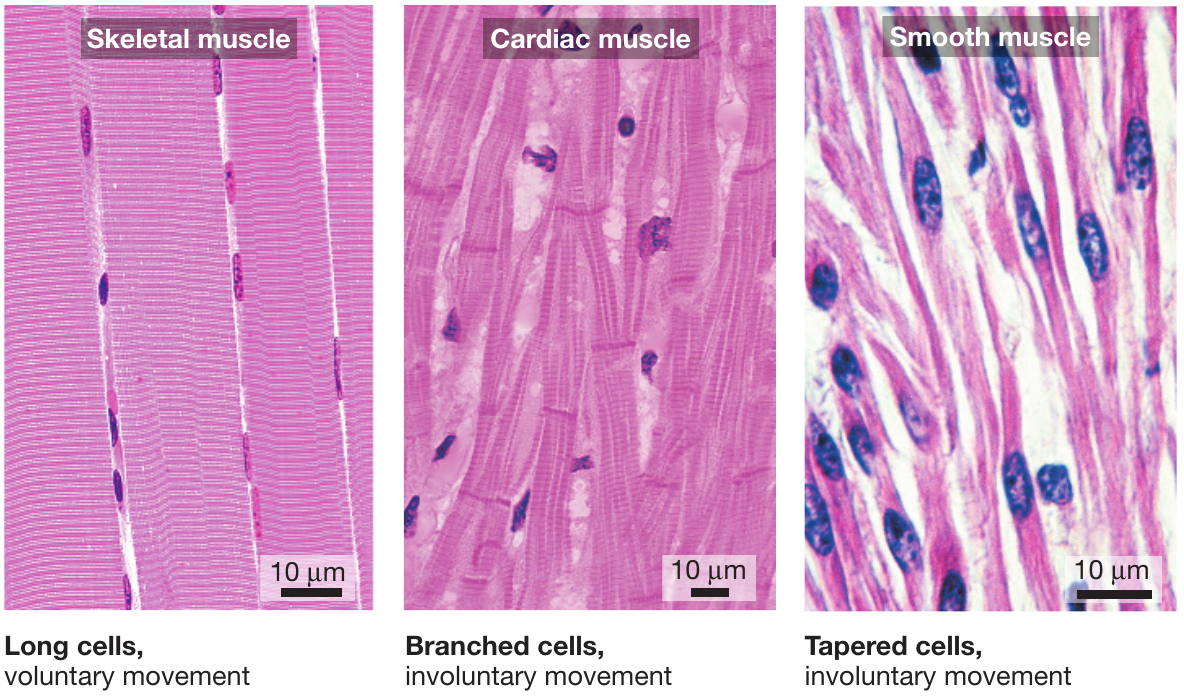
\includegraphics[scale=0.4]{images/muscle-types.png}}
        \end{itemize}
        \item \textbf{Epithelial tissues}: tissue that covers the outside of the body, line the inner surface of many organs, and form glands.
        \begin{itemize}
            \item \textbf{Organ}: a structure that serves a specialized function and consists of two or more tissues
            \item \textbf{Gland}: an organ that secretes specific molecules or solutions such as hormones or digestive enzymes.
            \item \textbf{Apical}: faces away from other tissues and toward the environment
            \item \textbf{Basolateral}: faces the interior of the animal and connects to connective tissues.
            \item \textbf{Basal lamina}: the connection made by a layer of fibers on the basolateral side.
        \end{itemize}
        \item \textbf{Organ system }: m consists of groups of tissues and organs that work together to perform one or more functions.
    \end{itemize}
}\end{secbox}

\hypertarget{39.3}{}
\begin{secbox}{\hyperlink{39}{How Does Body Size Affect Animal Physiology?}}{
    \begin{itemize}
        \item \textbf{Metabolic rate}: the overall rate of energy consumption by an individual.
        \item \textbf{Basal metabolic rate (BMR)}: the rate at which an animal consumes oxygen while at rest, with an empty stomach, under normal temperature and moisture conditions.
        \item \textbf{Gills}:  organs that allow the exchange of gases and dissolved substances between the animals’ blood and the surrounding water.
        \item \textbf{Adaptations for increased surface area}:
        \begin{itemize}
            \item \textbf{Flattening}: Fish have gill lamellae---thin sheets of epithelial cells that provide the gill with an extremely high surface area relative to its volume.
            \item \textbf{Folding}: portions of the digestive tract where nutrients are transported into the body, the surface of the structure is folded. Extending from these folds are narrow projections called villi.
            \item \textbf{Branching}: a highly branched network of small, thin-walled blood vessels called capillaries, which are the sites where gases, nutrients, and waste products diffuse into and out of blood, and branching greatly increases their surface area.\par 
            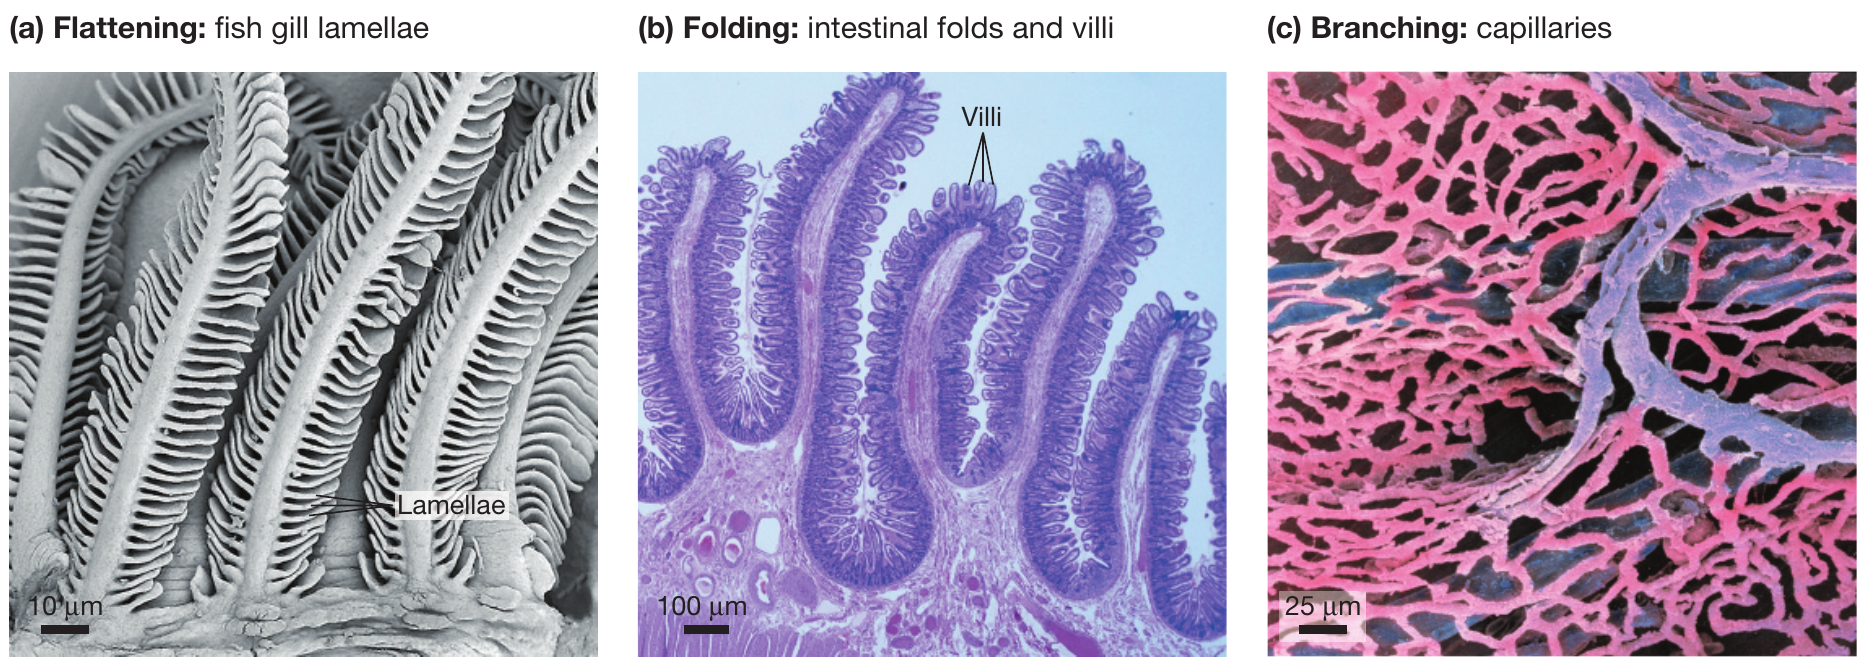
\includegraphics[width=\linewidth]{images/gills.png}
        \end{itemize}
    \end{itemize}
}\end{secbox}

\hypertarget{39.4}{}
\begin{secbox}{\hyperlink{39}{Homeostasis}}{
    \begin{itemize}
        \item \textbf{Homeostasis}: stability in the chemical and physical conditions within an organism’s cells, tissues, and organs.
        \item \textbf{Regulate}: to actively maintain relatively constant internal conditions even when the environment fluctuates.
        \item Epithelia are responsible for forming an internal environment that can be dramatically different from the external environment and for allowing physical and chemical conditions inside an animal to be maintained at relatively constant levels.
        \item \textbf{Homeostatic system:}:A homeostatic system consists of three general components: a sensor, an integrator, and an effector.
        \item \textbf{Hypothalamus}:a receptor region in the brain that responds to changes in blood temperature.
    \end{itemize}
}\end{secbox}

\hypertarget{39.5}{}
\begin{secbox}{\hyperlink{39}{Thermoregulation: A Closer Look}}{
    \begin{itemize}
        \item \textbf{Thermoregulatory strategies:}:conduction, convection, radiation, and evaporation.
        \begin{itemize}
            \item \textbf{Endotherm}: produces heat.
            \item \textbf{Ectotherm}: relies on heat.
            \item \textbf{Homeotherms}: keep their body temperature constant
            \item \textbf{Poikilotherms}: allow their body temperature to rise or fall depending on environmental conditions.
            \item \textbf{Torpor}: reduction of metabolic rate and that allows body temperature to drop, a form of poikilothermy.
            \item \textbf{Hibernation}: Extended periods of Torpor. 
        \end{itemize}
        \item \textbf{Countercurrent exchanger}: fluids that flow through adjacent pipes in opposite directions to reduce heat loss.
    \end{itemize}
}\end{secbox}   

\hypertarget{39.r}{}
\begin{probbox}{\hyperlink{39}{Chpater 39: Review}}{
    \hyperlink{39.1}{Form, Function, and Adaptation}
    \begin{itemize}
            \item Animal structures and their functions represent adaptations, which are heritable traits that improve survival and reproduction in a certain environment.
            \item Adaptations involve trade-offs, or inescapable compromises between traits.
            \item Acclimatization is a reversible response to the environment that improves physiological function in that environment.
        \end{itemize}
    \hyperlink{39.2}{Tissues, Organs, and Systems}
    \begin{itemize}
            \item Animal cells with a common function are grouped together into
            four general types of tissue: connective tissue, nervous tissue, muscle tissue, and epithelial tissue.
            \item Organs are structures that are composed of two or more tissues that together perform specific tasks.
            \item Organ systems comprise organs that work together in an integrated fashion to perform one or more functions.
    \end{itemize}
    \hyperlink{39.3}{How Does Body Size Affect Animal Physiology?}
    \begin{itemize}
            \item Large animals have smaller surface area/volume ratios than small animals. As animals grow, their volume increases more rapidly than their surface area. 
            \item Large animals have low mass-specific metabolic rates, in keeping with their relatively small surface area for exchanging the oxygen and nutrients required to support metabolism and the wastes and heat produced by metabolism.
            \item The relatively high surface area of small animals means that they lose heat extremely rapidly.
    \end{itemize}
    \hyperlink{39.4}{Homeostasis}
    \begin{itemize}
            \item Homeostasis refers to relatively constant physical and chemical conditions inside the body. 
            \item Homeostasis in a fluctuating environment is usually achieved by regulation. 
            \item Animals have set points, or target values, for various body parameters. When a parameter is not at its set point, negative feedback occurs. Responses to negative feedback return the parameter to the set point and result in homeostasis. 
            \item Most animals have a set point for body temperature. If an individual overheats, it may pant, sweat, or seek a cool environment; if an individual is cold, it may shiver, bask in sunlight, or fluff its fur or feathers.
        \end{itemize}
    \hyperlink{39.5}{Thermoregulation: A Closer Look}
    \begin{itemize}
            \item Animals vary from endothermic to ectothermic and from homeothermic to poikilothermic. 
            \item Endotherms can be active in cold environments but must obtain a lot of energy to fuel their metabolism. Ectotherms do not require as much energy, but their activity depends on environmental temperature. 
            \item Countercurrent heat exchangers have vessels in close contact that carry warm and cool fluids in opposite directions.
    \end{itemize}        
}\end{probbox}
%\endgroup
%  ^^^^^^^^^^^^^^^^^^^^^^^^^^^^^^^^^^   Chapter 39   ^^^^^^^^^^^^^^^^^^^^^^^^^^^^^^^^^^ %   
%%%%%%%%%%%%%%%%%%%%%%%%%%%%%%%%%%%%%%%%%%%%%%%%%%%%%%%%%%%%%%%%%%%%%%%%%%%%%%%%%%%%%%%%%

%%%%%%%%%%%%%%%%%%%%%%%%%%%%%%%%%%%%%%%%%%%%%%%%%%%%%%%%%%%%%%%%%%%%%%%%%%%%%%%%%%%%%%%%%
%  vvvvvvvvvvvvvvvvvvvvvvvvvvvvvvvvvv   Chapter 40   vvvvvvvvvvvvvvvvvvvvvvvvvvvvvvvvvv %
%\begingroup

\clearpage

\renewcommand{\thetitle}{\hypertarget{40}{Water and Electrolye Balance}}
\rfoot{\hyperlink{40}{40 --- \thepage}}
\hypertarget{40}{}
\setcounter{section}{40}

\begin{chapbox}{\hyperlink{home}{Chapter 40: Water and Electrolyte}}
    \begin{enumerate}
        \item \hyperlink{40.1}{Osmoregulation and Exertion}
        \item \hyperlink{40.2}{Water and Electrolyte in Marine Fishes}
        \item \hyperlink{40.3}{Water and Electrolyte in Freshwater Fishes}
        \item [5.] \hyperlink{40.5}{Water and Electrolyte in Vertebrates}
        \item [--] \hyperlink{40.r}{Review}
    \end{enumerate}
\end{chapbox}

\hypertarget{40.1}{}
\begin{secbox}{\hyperlink{40}{Osmoregulation and Exertion}}{
    \begin{itemize}
        \item \textbf{Electrolyte}: compound that dissociates into ions when dissolved in water. Electrolytes got their name because they conduct electrical current.        
        \item \textbf{Osmosis}: movement of water down its gradient across a semi­ permeable membrane
        \item \textbf{Osmoregulation}:is the process by which organisms control the concentration of water and solutes in their bodies.
        \item \textbf{Osmoconformers}: animals with concentrations of electrolytes and other solutes that match those of the sea.
        \item \textbf{Isosmotic}: solute concentrations inside and outside these animals are equal.
        \item \textbf{Osmoregulators}: most marine invertebrates, marine and fresh­ water bony fishes and terrestrial animals. These organisms actively regulate osmolarity inside their bodies to achieve homeostasis. 
        \item \textbf{Hyperosmotic}: the solution outside the body has a higher solute concentration than the solution inside.
        \item \textbf{Hyposmotic}: higher solute concentration than the freshwater outside
        \item \textbf{Aquaporins}: specialized membrane channels where water follows by osmosis due to cells that transport ions and that set up an osmotic gradient.
        \item \textbf{Ammonia}: the result of excess amino acids and nucleic acids when broken down in catabolic reactions and of which animals must secret since it raises the pH of cells. 
        \item \textbf{Urea}: a much less toxic compound created by enzyme­-catalyzed reactions of ammonia.
        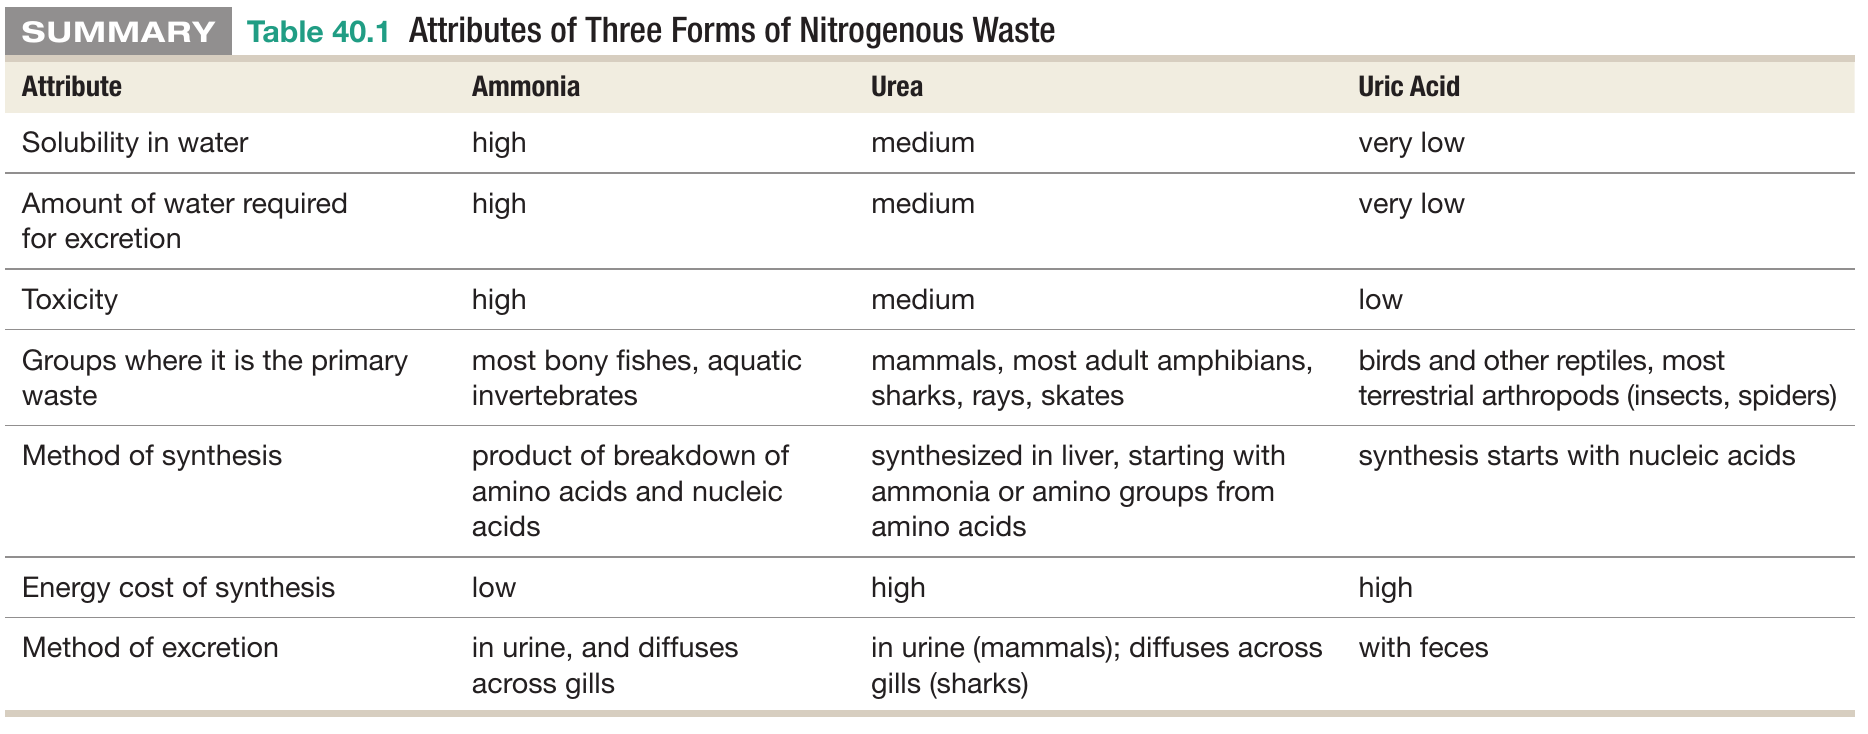
\includegraphics[width=\linewidth]{images/waste.png}
    \end{itemize}
}\end{secbox}

\hypertarget{40.2}{}
\begin{secbox}{\hyperlink{40}{Water and Electrolyte in Marine Fish}}{
    \begin{itemize}
        \item \textbf{Rectal gland}: an gland in sharks that secretes a concentrated salt solution.
        \item \textbf{Ouabain}: toxic to animals because it binds to Na+/K+­ATPase and prevents it from functioning and strong evidence that Na+/K+­ATPase is essential for salt excretion.
        \item \textbf{Interstitial fluid}: the extra-cellular fluid surrounding the rectal gland.
    \end{itemize}
}\end{secbox}

\hypertarget{40.3}{}
\begin{secbox}{\hyperlink{40}{Water and Electrolyte in Freshwater Fish}}{
    \begin{itemize}
        \item \textbf{Osmoregulatory cells may be in different locations}: when osmotic stress changes, the structure of the gill epithelium changes. Specifically, active pumping of ions takes place in different populations of cells in seawater and freshwater.        
        \item \textbf{Different forms of Na\(^+\)/K\(^+\)-ATPase may be activated}: the form activated when salmon are in seawater differs from the one activated when they are in freshwater.
        \item \textbf{The orientation of key transport proteins “flips.”}: When the fish are in seawater, the protein is located in the basolateral membrane of chloride cells. But when they are in freshwater, the protein is located in the apical membrane.
    \end{itemize}
}\end{secbox}

\hypertarget{40.5}{}
\begin{secbox}{\hyperlink{40}{Water and Electrolyte in Vertebrates}}{
    \begin{itemize}
        \item \textbf{Kidney}: the key organ of the urinary system osmoregulation primally occurs.
        \item \textbf{Ureter}: a long tube where the urine that forms in the kidney is transported.
        \item \textbf{Bladder}: the storage organ urine in the ureter is transported to. 
        \item \textbf{Urethra}: where urine is transported from bladder to the body surface.
        \item \textbf{Nephron}: small structures that are the basic functional unit of the
        kidney and makes up most of the kidney’s mass. Nephrons work involved in maintaining water and electrolyte balance.
        f\item \textbf{Cortex}: outer region of the an organ. 
        \item \textbf{Medulla}: the kidney’s inner region.
        \item \textbf{The Mammalian Kidney:}: To move water, cells in the kidney set up a strong osmotic gradient in the interstitial fluid surrounding the nephrons. By regulating these gradients and specific channel proteins, kidney cells exert precise control over loss or retention of water and electrolytes.
        \item \textbf{Renal Corpuscle}: a filtration device where urine formation begins. The renal corpuscle forms a capsule that encloses a cluster of capillaries called a \textbf{glomerulus}
        \item \textbf{Bowman's capsule}: region of the nephron that surrounds the glomerulus
        \item \textbf{Proximal tubule}: where filtrate reabsorption begins after leaving the Bowman's capsule. 
        \item \textbf{Microvilli}: small hairs that greatly increase the surface area of this epithelial cells of the proximal tubule.
        \item \textbf{Loop of Henle}: the location to which fluid that emerges from the proximal tubule flows to. In about 20 percent of the nephrons present in a human kidney, the loop is long and plunges from the cortex of the kidney deep into the medulla.
        \item The loop of Henle has three distinct regions: the descending limb, the thin ascending limb, and the thick ascending limb.
        \item \textbf{A Comprehensive View of the Loop of Henle:}: Movement of NaCl from the ascending limb into surrounding tissue increases the osmolarity of the fluid out­ side the descending limb, which results in an outward flow of water across the water­permeable epithelium of the descending limb, via osmosis. This loss of water in the descending limb increases the osmolarity of the fluid entering the ascending limb. The high concentration of salt in the fluid at the base of the ascending limb trig­ gers a passive flow of ions out—reinforcing the osmotic gradient.\par
        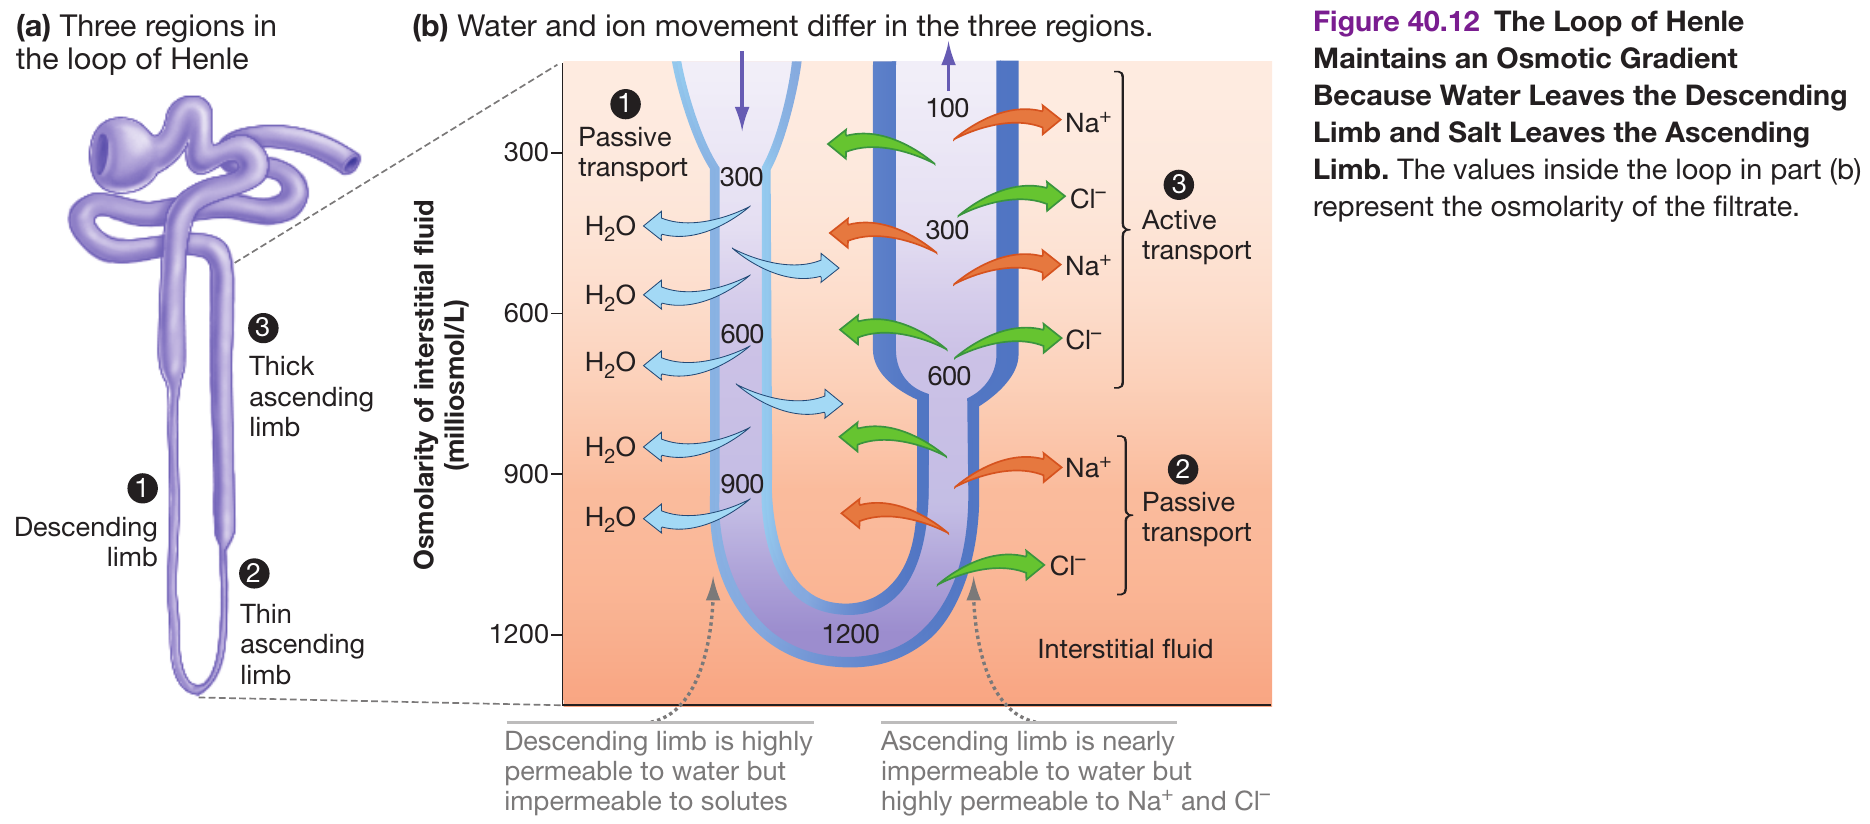
\includegraphics[width=\linewidth]{images/loop-of-henle.png}
        \item \textbf{Vasa recta}: a network of blood vessels that runs along the loop of henle where water and electrolytes that are reabsorbed are returned to the bloodstream instead of being excreted in urine.
        \item the system created by the nephron, vasa recta, and collecting duct results in the creation and maintenance of a strong osmotic gradient with the minimum possible expenditure of energy.
        \item \textbf{Hormones Involved}
            \begin{itemize}
                \item If Na+ levels in the blood are low, the adrenal glands release the hormone \textbf{aldosterone}, which leads to activation of sodium.
                \item  If an individual is dehydrated, the brain releases \textbf{antidiuretic hormone (ADH)}.
            \end{itemize}
        \item \textbf{Cloaca}: a cavity into which the urinary, gastrointestinal, and reproductive tracts all empty. Reptiles are able to absorb water from urine across the wall of the cloaca into the bloodstream. Eventually, a semisolid uric acid paste is excreted along with the feces.
    \end{itemize}
}\end{secbox}

\hypertarget{40.r}{}
    \begin{probbox}{\hyperlink{40}{Chaper 40: Review}}{
        \hyperlink{40.1}{Osmoregulation and Exertion}
        \begin{itemize}
            \item Solutes move across membranes via passive transport, facilitated diffusion, or active transport. Water moves across membranes by osmosis. 
            \item In most animals, epithelial cells that selectively transport water and electrolytes are responsible for homeostasis. 
            \item The mechanisms involved in regulating water and electrolyte balance vary widely among animal groups because different habitats present different types of osmotic stress.
            \item The type of nitrogenous waste excreted by an animal is affected by its phylogeny and its habitat type. Most fishes excrete ammonia; mammals and most adult amphibians excrete urea; and insects and reptiles excrete uric acid.
        \end{itemize}
        \hyperlink{40.2}{Water and Electrolyte in Marine Fishes}
        \begin{itemize}
            \item Seawater is strongly hyperosmotic to the tissues of marine bony fishes, so they tend to lose water by osmosis and gain electrolytes by diffusion. 
            \item Marine bony fishes are osmoregulators, whereas cartilaginous fishes including sharks are osmoconformers. 
            \item Epithelial cells in the shark rectal gland and in the gills of marine bony fishes excrete excess salt using Na\(^+\)/K\(^+\)­ATPase and Na\(^+\)/Cl\(^+\)/K\(^+\) cotransporters located in the basolateral membrane. 
            \item Similar salt­excreting cells also exist in the salt glands of marine birds and other reptiles and in the kidneys of mammals.
        \end{itemize}
        \hyperlink{40.3}{Water and Electrolyte in Freshwater Fishes}
        \begin{itemize}
            \item Freshwater is strongly hyposmotic to the blood of freshwater fishes, so they tend to gain water by osmosis and lose electrolytes by diffusion. 
            \item Epithelial cells in the gills of freshwater fishes import ions using Na\(^+\)/K\(^+\)­ATPase located in the basolateral membrane and Na\(^+\)/Cl\(^-\)/K\(^+\) cotransporters located in the apical membrane.
        \end{itemize}
        \hyperlink{40.5}{Water and Electrolyte in Vertebrates} 
        \begin{itemize}
            \item Nephrons in the vertebrate kidney form a filtrate in the renal corpuscle and then reabsorb valuable nutrients, electrolytes, and water in the proximal tubule. 
            \item A solution containing urea and electrolytes flows through the loop of Henle of mammalian kidneys, where changes in the permeability of epithelial cells to water and salt—along with active transport of salt—create a steep osmotic gradient. 
            \item Antidiuretic hormone increases the water permeability of the collecting duct, causing water to be reabsorbed along the osmotic gradient and hyperosmotic urine to be produced. 
            \item The nephrons of fishes, amphibians, and non­avian reptiles do not have loops of Henle and therefore cannot produce urine that is hyperosmotic to the body fluids. However, some of these vertebrates can produce hyperosmotic urine by reabsorbing water from the cloaca or bladder.
        \end{itemize}    
    }\end{probbox}
%\endgroup
%  ^^^^^^^^^^^^^^^^^^^^^^^^^^^^^^^^^^   Chapter 40   ^^^^^^^^^^^^^^^^^^^^^^^^^^^^^^^^^^ %  
%%%%%%%%%%%%%%%%%%%%%%%%%%%%%%%%%%%%%%%%%%%%%%%%%%%%%%%%%%%%%%%%%%%%%%%%%%%%%%%%%%%%%%%%%

%%%%%%%%%%%%%%%%%%%%%%%%%%%%%%%%%%%%%%%%%%%%%%%%%%%%%%%%%%%%%%%%%%%%%%%%%%%%%%%%%%%%%%%%%
%  vvvvvvvvvvvvvvvvvvvvvvvvvvvvvvvvvv   Chapter 41   vvvvvvvvvvvvvvvvvvvvvvvvvvvvvvvvvv %
%\begingroup

\clearpage

\renewcommand{\thetitle}{\hypertarget{41}{Nutrition}}
\rfoot{\hyperlink{41}{41 --- \thepage}}
\hypertarget{41}{}
\setcounter{section}{41}

\begin{chapbox}{\hyperlink{home}{Chapter 41: Nutrition}}
    \begin{enumerate}
        \item \hyperlink{41.1}{Nutritional Requirements}
        \item [3.]\hyperlink{41.3}{How are Nutrients Digested and Absorbed?}
        \item [4.]\hyperlink{41.4}{Nutritional Homeostasis}
        \item [i.]\hypertarget{41.r}{Review}
    \end{enumerate}
\end{chapbox}

\hypertarget{41.1}{}
\begin{secbox}{\hyperlink{41}{Nutritional Requirements}}{
    \begin{itemize}
        \item \textbf{Ingestion}: bringing in food.
        \item \textbf{Digestive tract}: also known as the alimentary canal or gastrointestinal (GI) tract.
        \item \textbf{Digestion}: breaking down food.
        \item \textbf{Absorption}: the uptake of specific ions and molecules across the epithelium that lines the digestive tract.
        \item \textbf{Essential nutrient}: are those that cannot be synthesized and must be obtained from the diet.\par 
        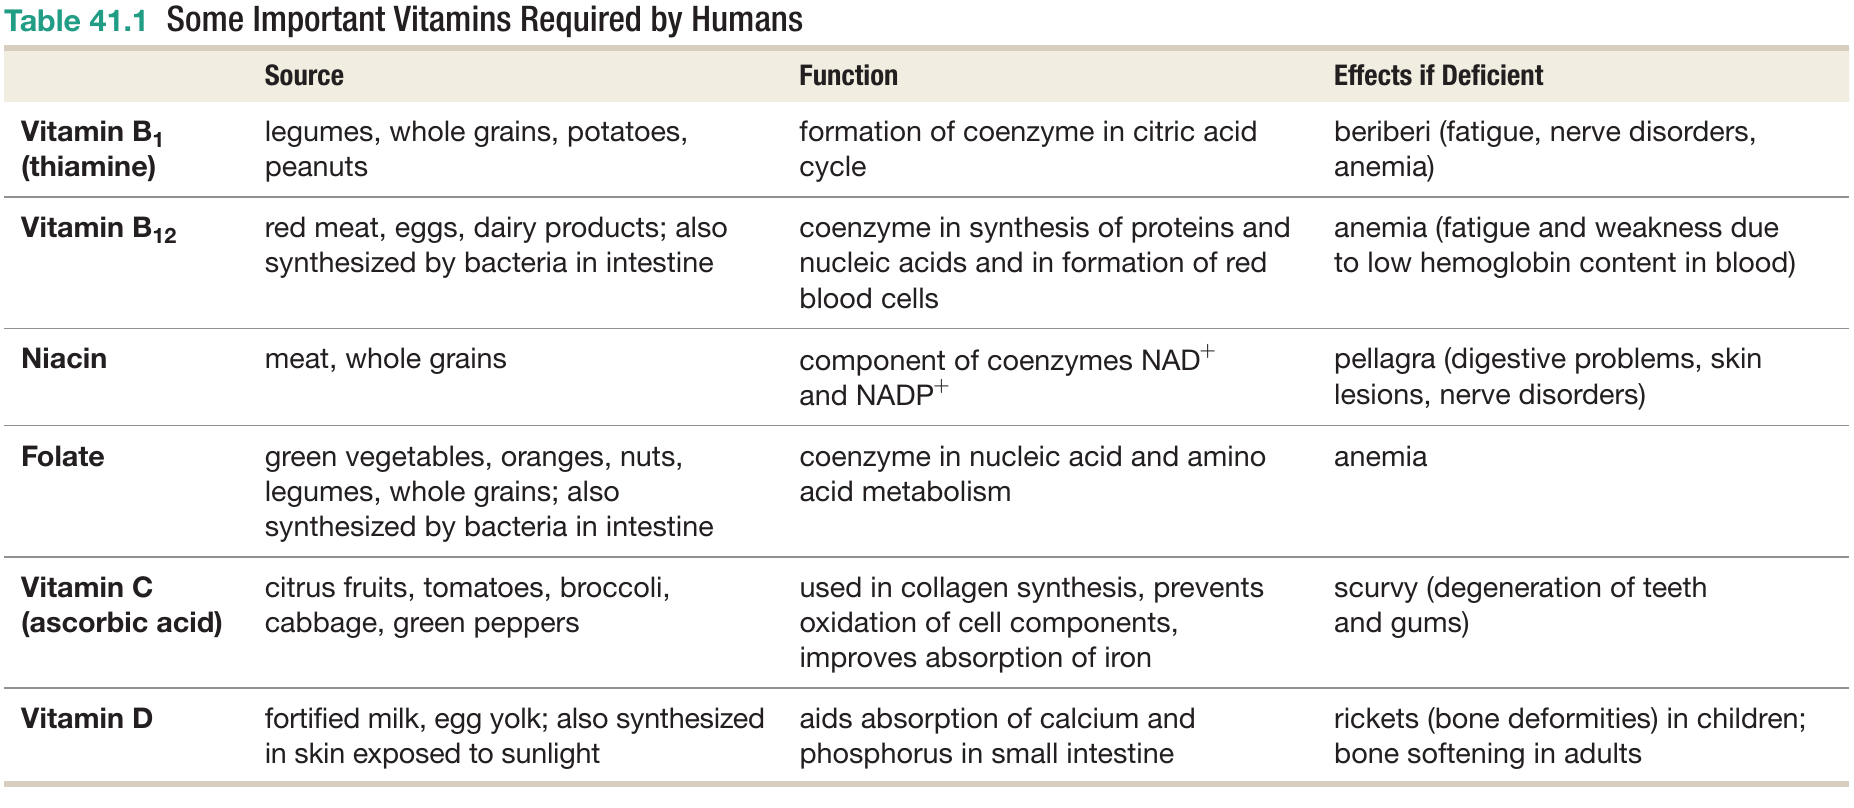
\includegraphics[width=\linewidth]{images/tbl41-1.png}\\
        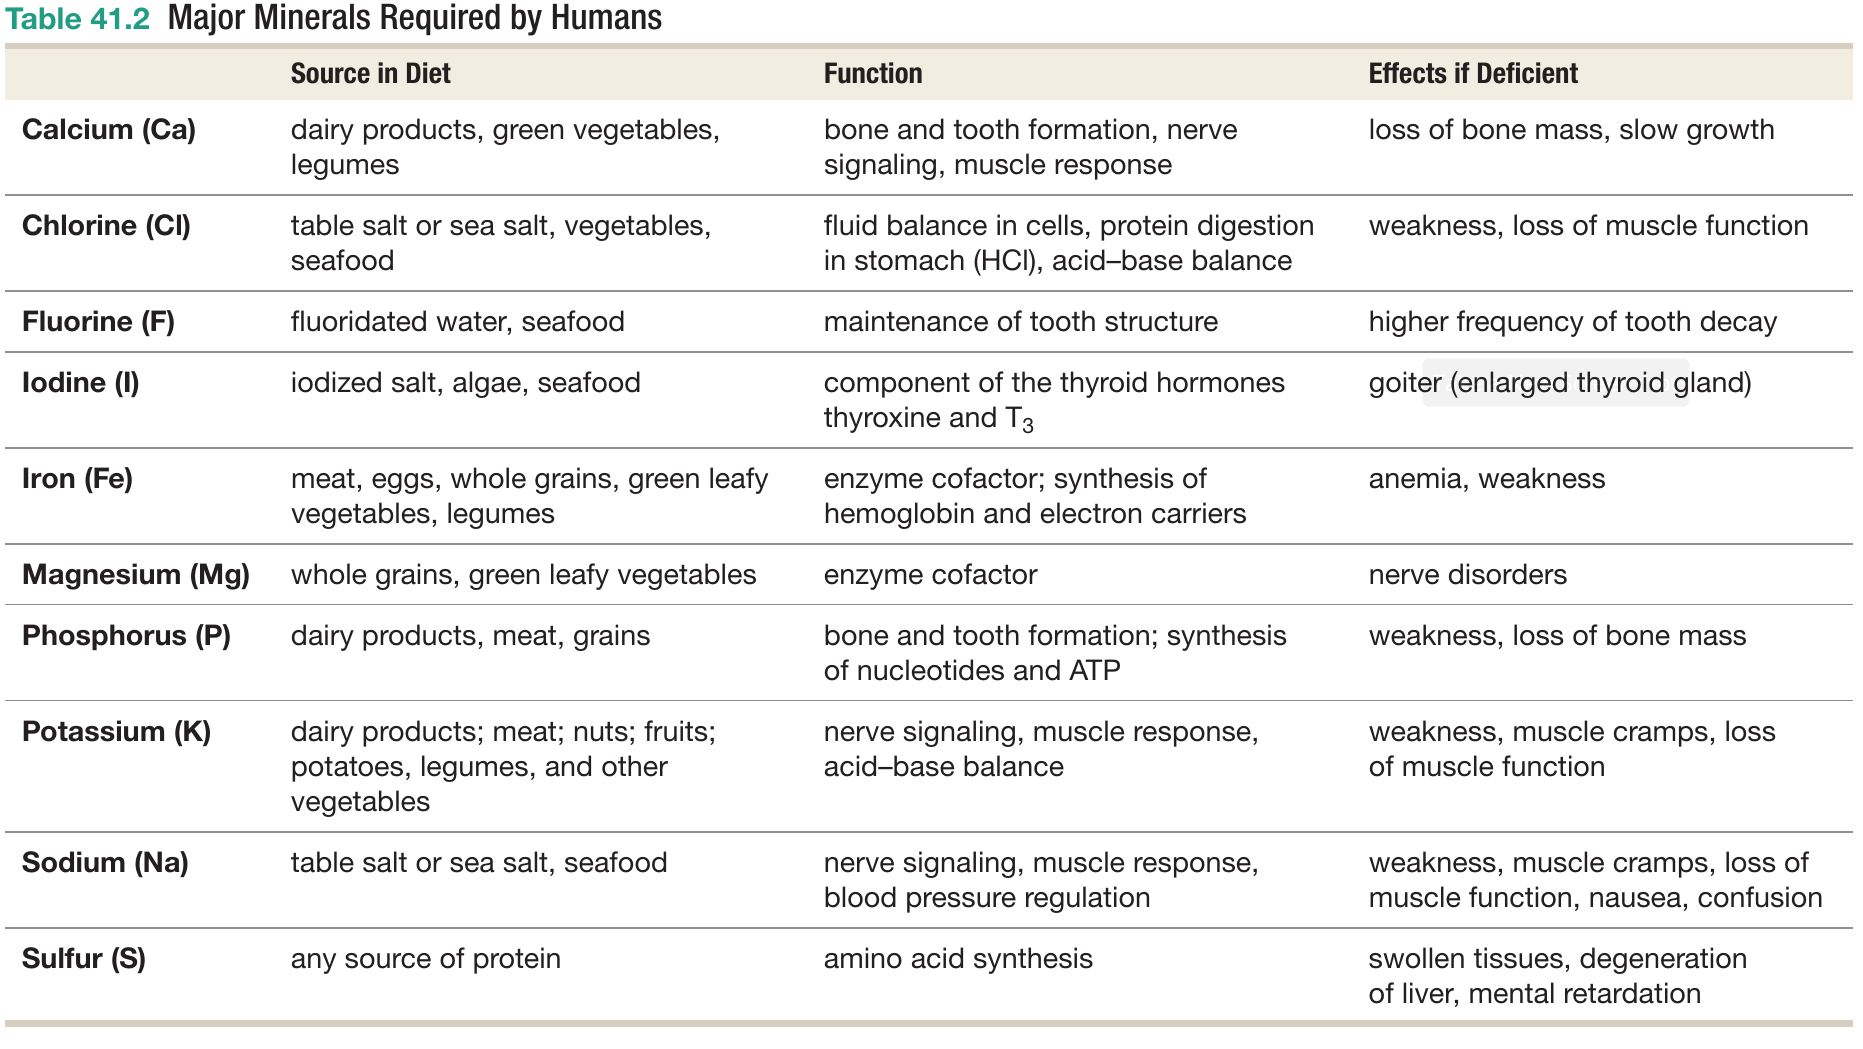
\includegraphics[width=\linewidth]{images/tbl41-2.png}
    \end{itemize}
}\end{secbox}

\hypertarget{41.3}{}
\begin{secbox}{\hyperlink{41}{How are Nutrients Digested and Absorbed?}}{
    \begin{itemize}
        \item \textbf{Incomplete digestive tracts}: a single opening, the mouth, through which the animal both ingests food and eliminates wastes.
        \item \textbf{Complete digestive tracts}: two openings—they start at the mouth and end at the anus.\par 
        \begin{center}
            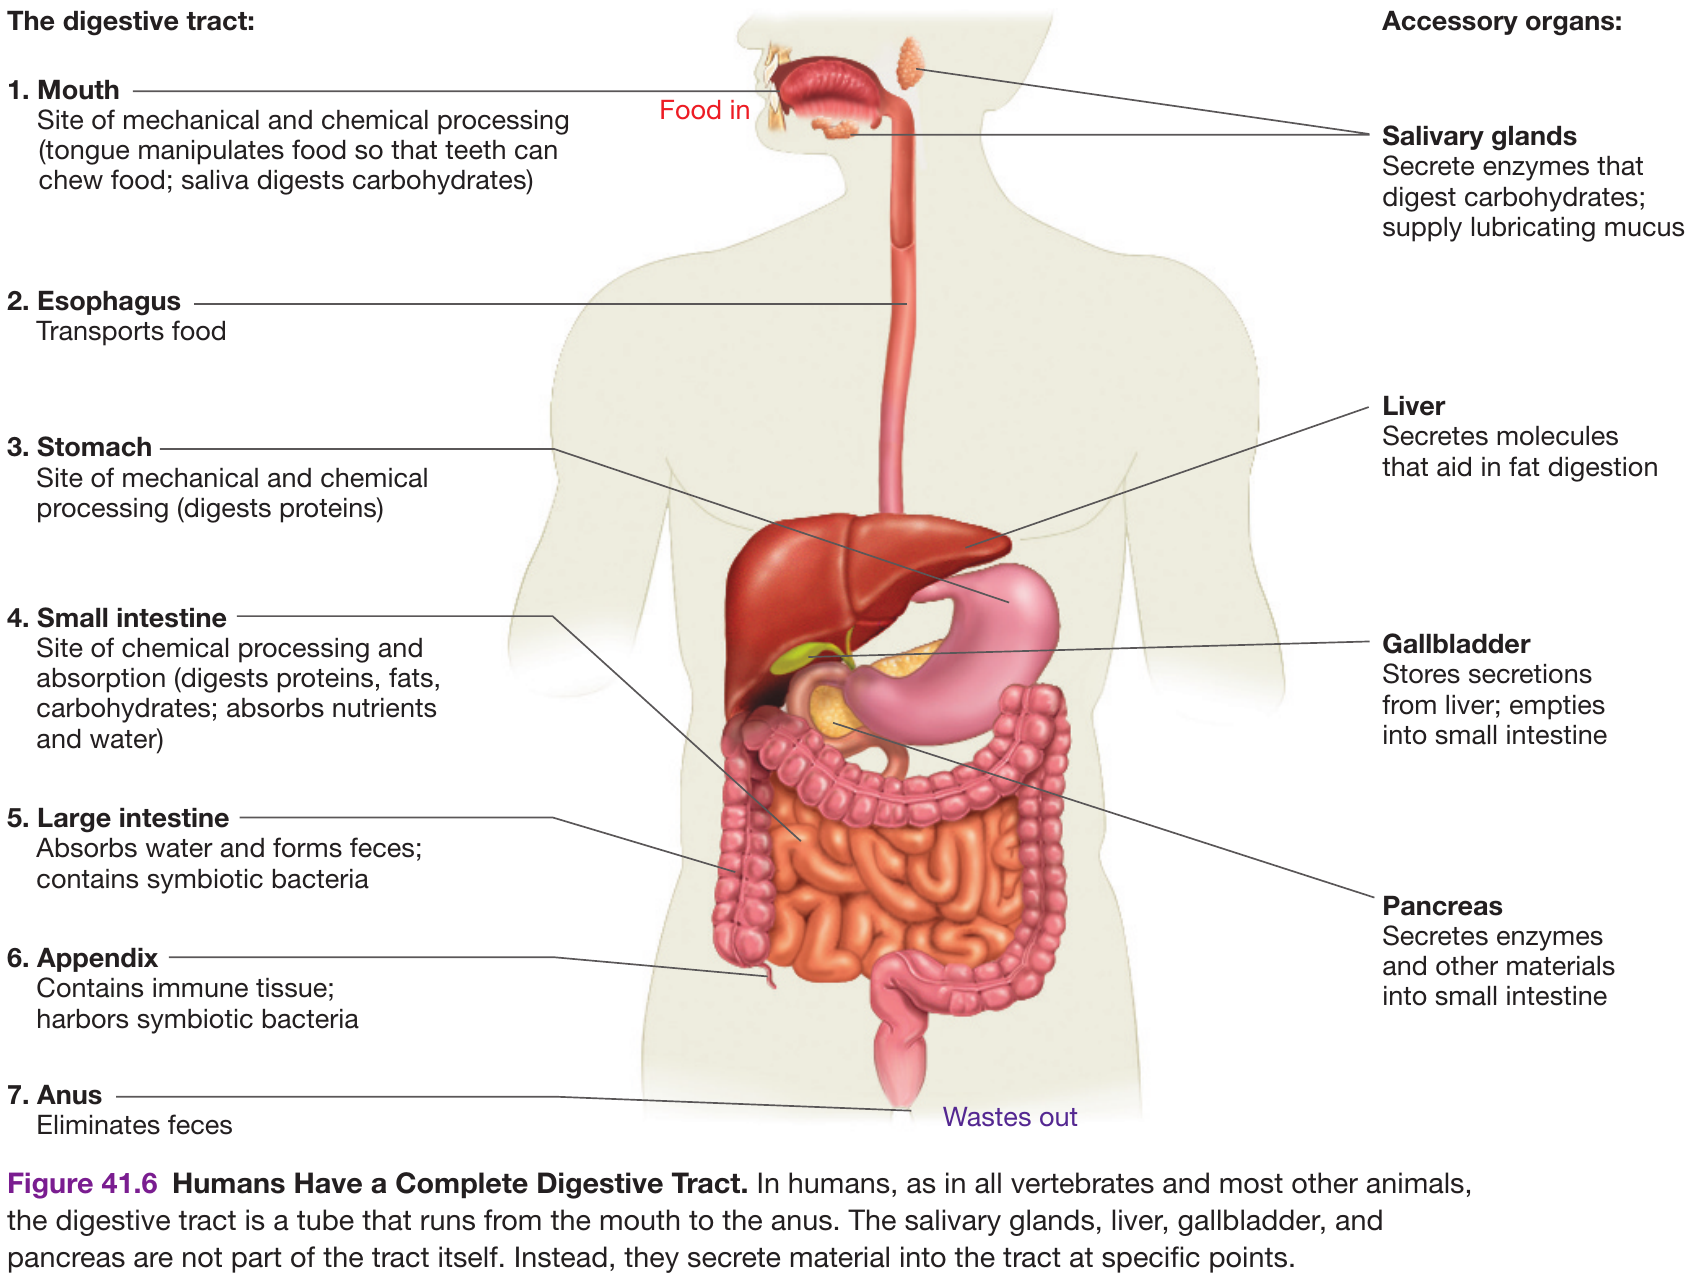
\includegraphics[scale=0.25]{images/digest.png}\\
            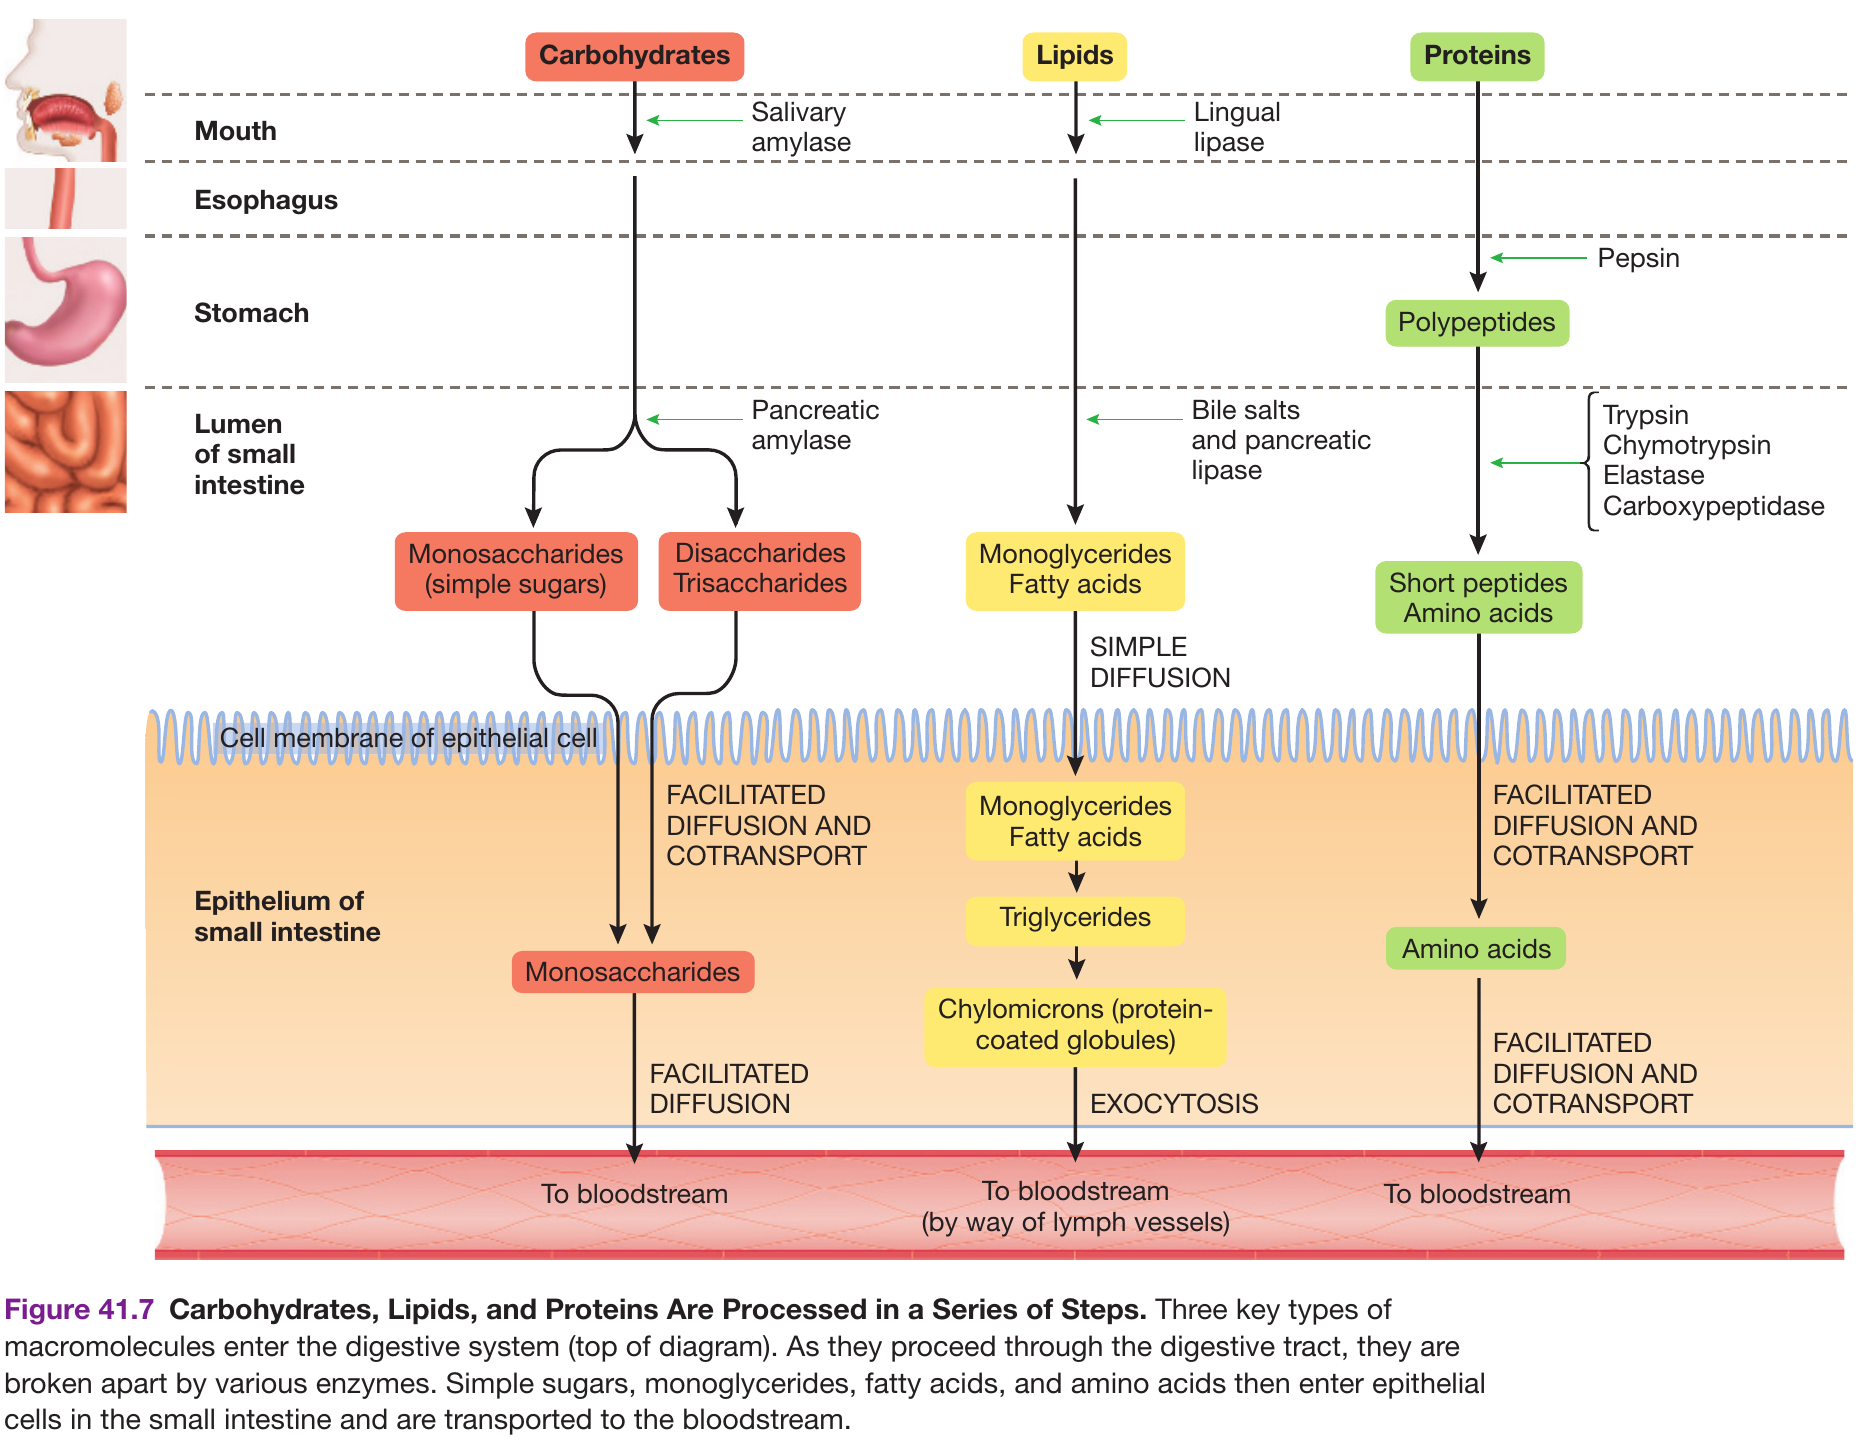
\includegraphics[scale=0.25]{images/digest-2.png}
        \end{center}
        \item \textbf{Feces}: the material remaining in the large intestine and excreted.
        \item \textbf{Salivary amylase}: the enzyme  responsible for starch digestion in the mouth
        \item \textbf{Lingual lipase}: which begins the digestion of lipids by breaking triglycerides into diglycerides and fatty acids.
        \item \textbf{Salivary glands}: glands in the mouth that not only secrete amylase but also produce the slimy substance called mucus.
        \item \textbf{Esophagus}: a muscular tube called that connects the mouth and stomach.
        \item \textbf{Peristalsis}: wave of muscular contractions called peristalsis propels food down the esophagus.
        \item \textbf{Crop}: where food can be stored and, in some cases, processed.
        \item \textbf{Stomach}:a tough, muscular pouch in the digestive tract, bracketed on both the superior and inferior ends by ringlike muscles called \textbf{sphincters}, which control the passage of material.
        \item \textbf{Pepsin}: enzyme that is responsible for digesting proteins in the stomach
        \item \textbf{Parietal cells}: the source of the HCl in gastric juice, which may have a pH as low as 1.5.
        \item \textbf{Mucous cell}: secretes additional mucus that is found in gastric juice. Mucus lines the gastric epithelium and protects the stomach from damage by HCl.
        \item \textbf{Carbonic anhydrase}: catalyzes the formation of carbonic acid (H2CO3) from carbon dioxide and water.
        \item \textbf{Ulcer}: an eroded area in an epithelium; it exposes the underlying tissues to damage
        \item \textbf{Ruminants}: the stomach is specialized for digesting cellulose instead of proteins.
        \item \textbf{Cellulase}: an enzyme capable of breaking the chemical bonds in cellulose, yielding glucose.
        \item \textbf{Small intestine}: a long tube that is folded into a com- pact space within the abdomen where most nutrients—along with large quantities of water—have been absorbed.
        \item \textbf{Villi}: fingerlike projections that cover the small intestine's tissue. Villi themselves have microvilli that protrude on the apical side. 
        \item \textbf{Lacteal}: lymphatic vessel that allows nutrients to quickly pass from epithelia to the body's transport system.
        \item \textbf{Proteases}:protein-digesting enzymes specific to certain types or configurations of amino acids in a polypeptide chain.
        \item \textbf{Pancreas}: an organ connected to the small intestine by the pancreatic duct that is responsible for production of proteases.
        \item \textbf{Trypsin}:triggers the activation of other proteases, such as chymotrypsin, elastase, and carboxypeptidase.
        \item \textbf{Hormone}: a chemical messenger that influences physiological processes at very low concentrations.
        \item \textbf{Secretin}: a hormone produced by the small intestine in response to the arrival of food from the stomach.
        \item \textbf{Cholecystokinin}: stimulates the secretion of digestive enzymes from the pancreas and the secretion of molecules from the gallbladder that aid in processing lipids.
        \item \textbf{Gastrin}: stimulates parietal cells to begin secreting HCl.
        \item \textbf{Pancreatic amylase}: continues the digestion of carbohydrates that began in the mouth.
        \item \textbf{Pancreatic lipase}: breaks certain bonds present in fats and results in the release of fatty acids and other small lipids.
        \item \textbf{Emulsification}: the process in which large fat globules
        that emerge from the stomach are broken up.
        \item \textbf{Liver}: organ that performs an array of functions related to digestion, and secreted in a complex solution called \textbf{bile}, which is stored in the \textbf{gallbladder} and contains bile salts used to break up lipids in plasma membranes.
        \begin{center}
            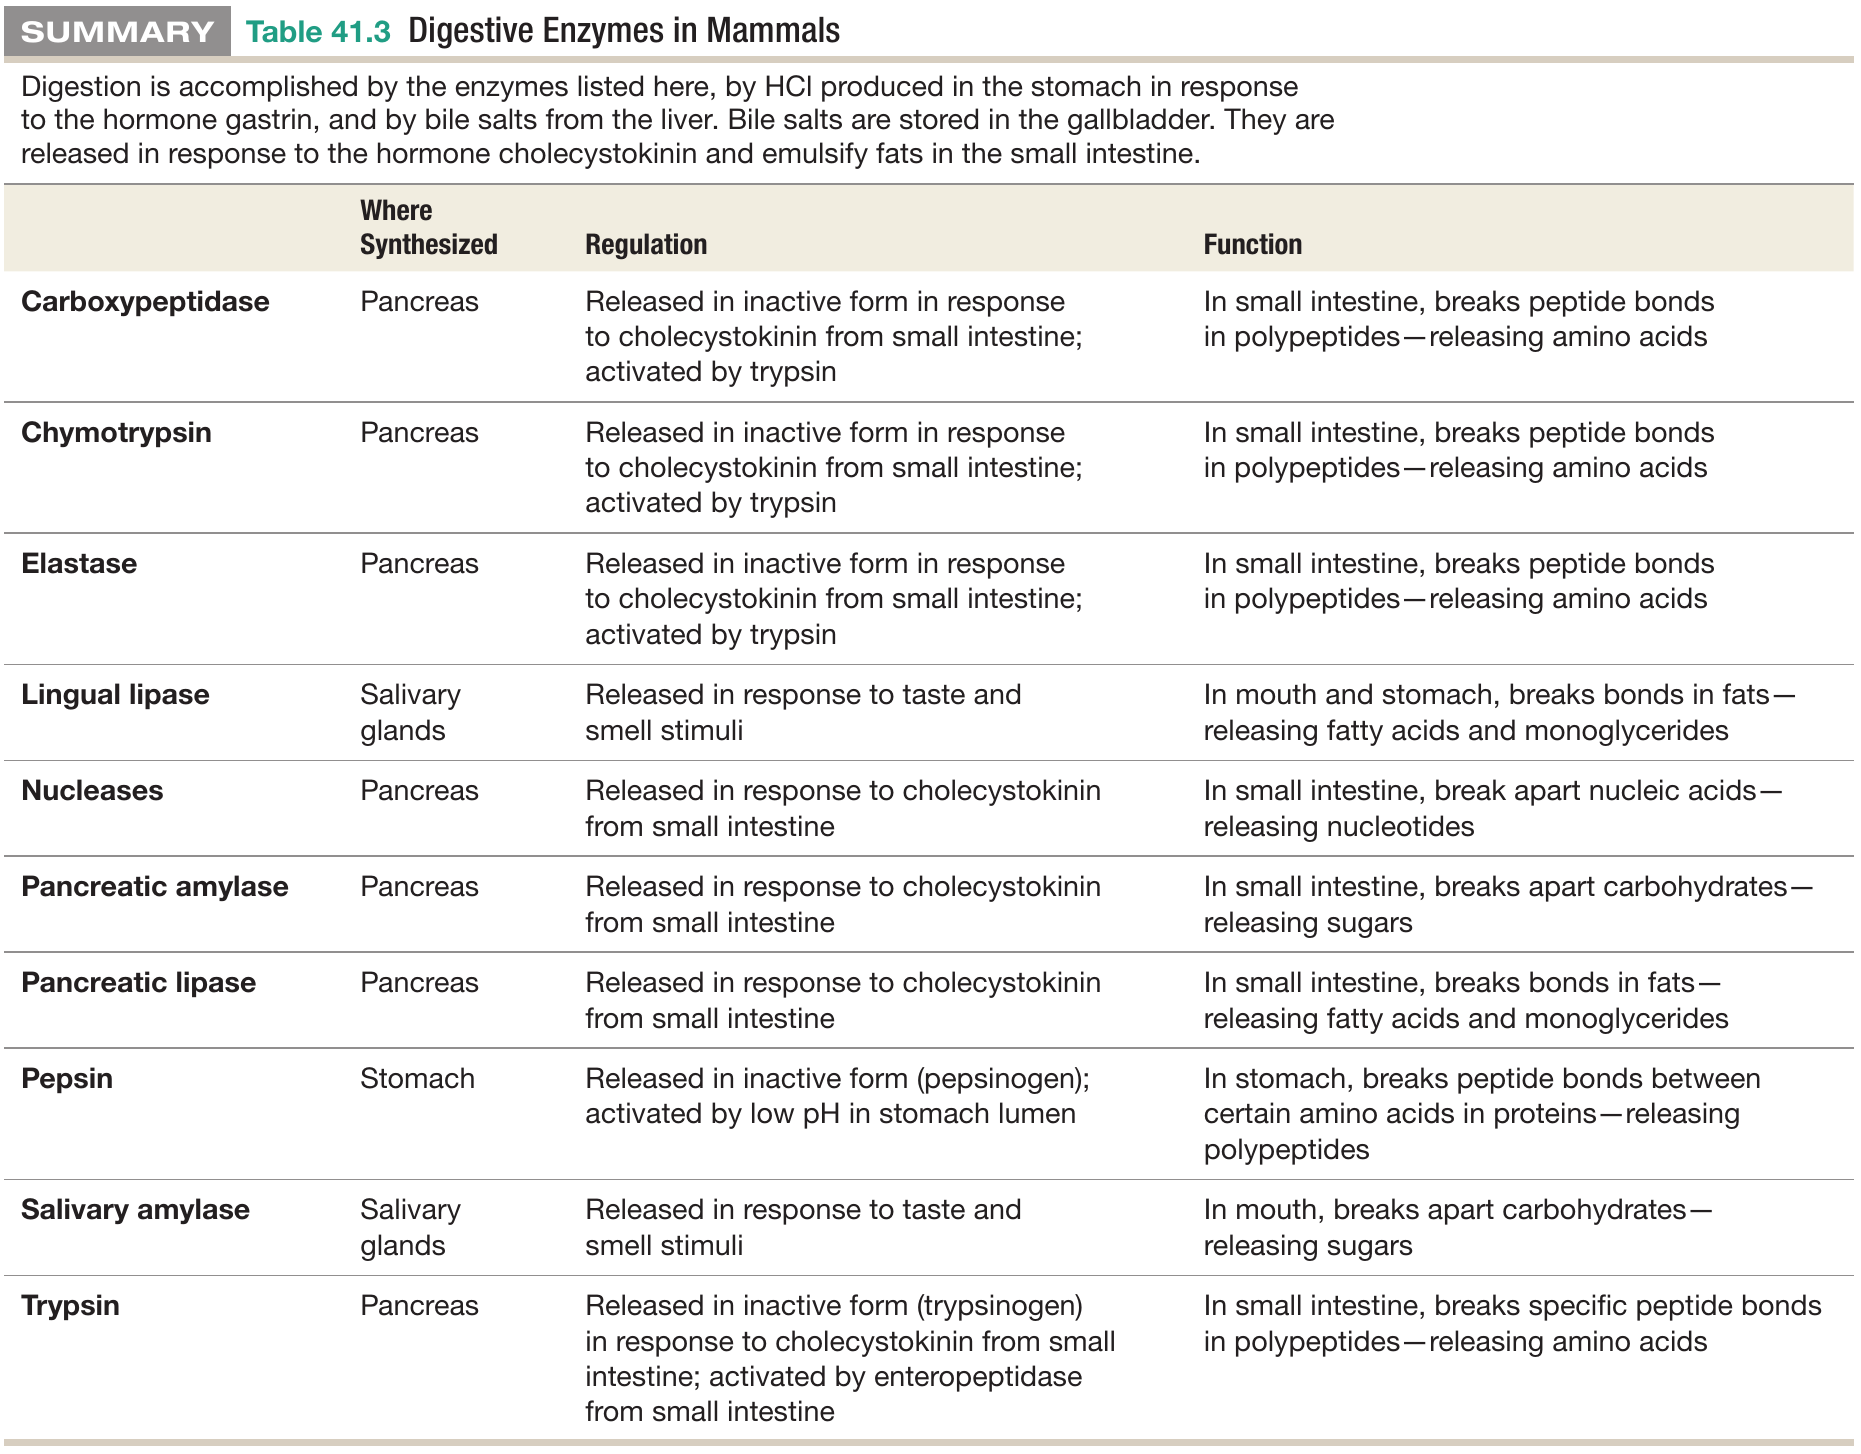
\includegraphics[scale=0.25]{images/tbl41-3.png}
        \end{center}
        \item \textbf{Large intestine}: form feces by absorbing additional water and compacting the wastes that remain.
        \item \textbf{Colon}: the main section of the large intestine.
        \item \textbf{Rectum}:the final part of the large intestine, until they can be eliminated.
        \item \textbf{Cecum}: a blind sac at the anterior end of the large intestine in some herbivores.
        \item \textbf{Appendix}: the function of the appendix has long been debated, either vestigial or a storage sac for symbiotic organisms. 
        \item \textbf{Coprophagy}: reabsorption of feces, allowing the animal to absorb more nutrients from food.
        \item \textbf{Cloaca}: an enlarged portion of the large intestine into which the reproductive tract also empties in the rectum of amphibians, reptiles, and birds. 
    \end{itemize}
}\end{secbox}

\hypertarget{41.4}{}
\begin{secbox}{\hyperlink{41}{Nutritional Homeostasis}}{
    \begin{itemize}
        \item \textbf{Diabetes mellitus}: abnormally high levels of glucose in their blood because cells cannot import the glucose. 
        \item \textbf{Insulin}: a hormone that is secreted by cells in the pancreas when blood glucose levels are too high.
        \item \textbf{Glucagon}: a hormone that causes liver cells catabolize stored glycogen and produce glucose via \textbf{gluconeogenesis}, the synthesis of glucose from non-carbohydrate compounds.
        \item \textbf{Diabetes mellitus}
            \begin{itemize} 
                \item type 1 does not synthesize sufficient insulin 
                \item type 2 are resistant to insulin, meaning that insulin does not effectively activate its receptor in target cells. 
                \item In both types, effector cells do not receive the signal that would result in a drop in blood glucose levels.
            \end{itemize}
        \item \textbf{Body mass index (BMI)}: a measure of obesity. BMI is calculated as body mass (in kilograms) divided by height (in meters) squared. A person with a BMI of 30 or higher is considered obese and has a far greater risk of developing type 2 diabetes mellitus than people with lower BMIs.
    \end{itemize}
}\end{secbox}

\hypertarget{41.r}{}
\begin{probbox}{\hyperlink{41}{Chapter 41: Review}}{
    \hyperlink{41.1}{Nutritional Requirements}
    \begin{itemize}
        \item The diets of animals include fats, carbohydrates, and proteins that provide energy; vitamins that serve as coenzymes and perform other functions; minerals that are used as components of enzyme cofactors or structural materials; and ions of electrolytes required for osmotic balance and normal membrane function. 
        \item Fats contain more energy (about 9 kcal/g) than carbohydrates or proteins (about 4 kcal/g), making fats an efficient way to store energy in the body.
    \end{itemize}
    \hyperlink{41.3}{How Are Nutrients Digested and Absorbed?}
    \begin{itemize}
        \item Most animals have a digestive tract that begins at the mouth and ends at the anus. 
        \item In many animals, chemical digestion of food begins in the mouth. In mammals, salivary amylase hydrolyzes bonds in starch and glycogen, and lingual lipase hydrolyzes bonds in fats. 
        \item Once food is swallowed, it is propelled down the esophagus by peristalsis. 
        \item Digestion continues in the stomach. In the human stomach, a highly acidic environment denatures proteins, and the enzyme pepsin begins the cleavage of peptide bonds that link amino acids. 
        \item Food passes from the stomach into the small intestine, where it is mixed with secretions from the pancreas and liver. 
        \item In the small intestine, carbohydrate digestion is continued by pancreatic amylase; fats are emulsified by bile salts and digested by pancreatic lipase; and protein digestion is completed by a suite of pancreatic proteases. 
        \item Cells that line the small intestine absorb the nutrients released by digestion. In many cases, uptake is driven by an electrochemical gradient established by Na\(^+\)/K\(^+\)-ATPase that favors the diffusion of Na\(^+\) into the cells. 
        \item As solutes leave the lumen of the small intestine and enter cells, water follows by osmosis. 
        \item Water reabsorption is completed in the large intestine, where feces form. 
        \item The structure of organs in the digestive tract varies widely among species, in ways that support processing of the food each species ingests.
    \end{itemize}
    \hyperlink{41.4}{Nutritional Homeostasis}
    \begin{itemize}
        \item Diabetes mellitus is a condition in which the level of glucose in the blood is abnormally high.
        \item Type 1 diabetes mellitus is caused by a defect in the production of insulin—a hormone secreted by the pancreas that promotes the uptake of glucose from the blood.
        \item Type 2 diabetes mellitus is characterized by a failure of cells to respond to insulin.
        \item The development of type 2 diabetes is correlated with obesity. The incidence of this disease has reached epidemic proportions in many populations.
    \end{itemize}
}\end{probbox}

%\endgroup
%  ^^^^^^^^^^^^^^^^^^^^^^^^^^^^^^^^^^   Chapter 41   ^^^^^^^^^^^^^^^^^^^^^^^^^^^^^^^^^^ %  
%%%%%%%%%%%%%%%%%%%%%%%%%%%%%%%%%%%%%%%%%%%%%%%%%%%%%%%%%%%%%%%%%%%%%%%%%%%%%%%%%%%%%%%%%

%%%%%%%%%%%%%%%%%%%%%%%%%%%%%%%%%%%%%%%%%%%%%%%%%%%%%%%%%%%%%%%%%%%%%%%%%%%%%%%%%%%%%%%%%
%  vvvvvvvvvvvvvvvvvvvvvvvvvvvvvvvvvv   Chapter 42   vvvvvvvvvvvvvvvvvvvvvvvvvvvvvvvvvv %
%\begingroup

\clearpage

\renewcommand{\thetitle}{\hypertarget{42}{Gas Exchange}}
\rfoot{\hyperlink{42}{42 --- \thepage}}
\hypertarget{42}{}
\setcounter{section}{42}

\begin{chapbox}{\hyperlink{home}{Chapter 42: Gas Exchange}}
    \begin{enumerate}
        \item \hyperlink{42.1}{The Resipitory and Circulatory System}
        \item \hyperlink{42.2}{Air and Water as Resipitory Media}
        \item \hyperlink{42.3}{Organs of Gas Exchange}
        \item \hyperlink{42.4}{How are Oxygen and Carbon Dioxide Transported in Blood?}
        \item \hyperlink{42.5}{Circulation}
        \item [--] \hyperlink{42.r}{Review}
    \end{enumerate}
\end{chapbox}

\hypertarget{42.1}{}
\begin{secbox}{\hyperlink{42}{The Resipitory and Circulatory System}}{
    \begin{itemize}
        \item [1.]\textbf{Ventilation}: the movement of air or water through a specialized gas exchange organ, such as a lung or gill.
        \item [2.]\textbf{Diffusion at the respiratory surface}: where O2 moves from the air or water into the blood and CO2 moves from the blood into the air or water
        \item [3.]\textbf{Circulation}: the transport of dissolved O2 and CO2 throughout the body—along with nutrients, wastes, and other types of molecules—via the circulatory system.
        \item [4.]\textbf{Diffusion at the tissues}: where O2 moves from the blood into the tissues and CO2 moves from the tissues into the blood.
        \item [5.]\textbf{Cellular respiration}: the cell’s use of O2 and production of CO2. In tissues, where cellular respiration has led to low O2 levels and high CO2 levels, gas exchange occurs between blood and cells.
        \item \textbf{Respiratory system}: the collection of cells, tissues, and organs responsible for gas exchange between the animal and its environment, or steps 1 and 2.
        \item \textbf{Circulatory system}: the system which moves O2, CO2, and other materials around the body. In many cases, a muscular heart propels a specialized, liquid transport tissue throughout the body via a system of vessels. 
    \end{itemize}
}\end{secbox}

\hypertarget{42.2}{}
\begin{secbox}{\hyperlink{42}{Air and Water as Resipitory Media}}{
    \begin{itemize}
        \item \textbf{Partial pressure}: the pressure of a particular gas in a mixture of gases.
        \item \textbf{Affects on Gas in Solution}
        \begin{itemize}
            \item Solubility of the gas in water
            \item Temperature of the water
            \item Presence of other solutes
            \item Partial pressure of the gas in contact with the water
        \end{itemize}
        \item \textbf{Affects on Oxygen in Solution}
        \begin{itemize}
            \item Habitats with large numbers of photosynthetic organisms tend to be relatively oxygen rich.
            \item Water near the surface has much higher oxygen content than water near the bottom of the same habitat under nonmoving conditions. 
            \item Shallow ponds and streams tend to be much better oxygenated than deep bodies of water because shallower bodies have a higher ratio of surface area to volume.
            \item Rapids, waterfalls, and breaking waves are the most highly oxygenated of all aquatic environments because a large surface area is exposed to the atmosphere as water splashes and because air bubbles are incorporated into the water.
        \end{itemize}
    \end{itemize}
}\end{secbox}

\hypertarget{42.3}{}
\begin{secbox}{\hyperlink{42}{Organs of Gas Exchange}}{
    \begin{itemize}
        \item \textbf{Fick’s law of diffusion} the rate of diffusion of a gas depends on five parameters: the solubility of  the gas in the aqueous film lining the gas exchange surface; the temperature; the surface area available for diffusion; the difference in partial pressures of the gas across the gas exchange surface; and the thickness of the barrier to diffusion 
        \item \textbf{Operculum}: the stiff flap of tissue that covers the gills.
        \item \textbf{Gill filament}: long, thin structures that extend from each gill arch. Each gill filament is composed of hundreds or thousands of \textbf{gill lamellae}. 
        \item \textbf{Tracheae (insect)}: an extensive system of air-filled tubes that connect to th exterior spiracles.
        \item \textbf{Spiracles}: openings in the exoskeleton that can be closed to minimize the loss of water by evaporation.
        \item \textbf{Trachea (human)}:  a tube that carries the inhaled air to narrower tubes called \textbf{bronchi}, which branch of into yet narrower tubes called \textbf{bronchioles}. All together these structures make up the lungs. 
        \item \textbf{Lungs}: the internal organs that are used for gas exchange. Terrestrial vertebrates—amphibians, reptiles (including birds), and mammals—have lungs, as do certain fishes and invertebrates.
        \item \textbf{Alveoli}: tiny sacs that make up the lungs of mammals. Each human has approximately 150 million alveoli. 
        \item \textbf{Positive pressure ventilation}: mechanism for pumping air used by frogs and other amphibians. Pushes air into lungs.
        \item \textbf{Negative pressure ventilation}: inverse of positive, pulling air into the lungs. 
        \item \textbf{Diaphragm}: a thin muscular sheet responsible for the change in volume be creating a by a downward motion and an expansion of the ribcage. 
        \item \textbf{Dead space}: air passages that are not lined by a respiratory surface.
    \end{itemize}
}\end{secbox}

\hypertarget{42.4}{}
\begin{secbox}{\hyperlink{42}{How are Oxygen and Carbon Dioxide Transported in Blood?}}{
    \begin{itemize}
        \item \textbf{Platelets}: cell fragments that act to minimize blood loss from ruptured blood vessels. They do so by releasing material that helps form the blockages known as clots 
        \item \textbf{White blood cells}: part of the immune system. They fight infections.
        \item \textbf{Red blood cells}: transport oxygen from the lungs to tissues throughout the body. 
        \item \textbf{Hemoglobin}: oxygen-carrying tetramer
        \item \textbf{Heme}: a nonprotein bound to the end of each chain on hemoglobin.
        \item \textbf{Oxygen–hemoglobin equilibrium curve}: a sigmoidal curve from the measurement of each successive oxygen molecule to a subunit of the hemoglobin molecule causes a conformational change in the protein that makes the remaining subunits much more likely to bind oxygen. The phenomenon is called \textbf{Cooperative binding}.
        \item \textbf{Bohr shift}: when the oxygen–hemoglobin equilibrium curve shifts to the right. This happens when pH declines or temperature increases.
    \end{itemize}
}\end{secbox}

\hypertarget{42.5}{}
\begin{secbox}{\hyperlink{42}{Circulation}}{
    \begin{itemize}
        \item \textbf{Open circulatory system}: a fluid connective tissue called
        hemolymph is actively pumped throughout the body in a limited
        system of vessels.
        \item \textbf{Heart}: organ that pumps hemolymph into vessels that empty into open, fluid-filled spaces
        \item \textbf{Closed circulatory system}: blood flows in a continuous
        circuit through a series of vessels in the body, under pressure
        generated by a heart. 
        \item \textbf{Arteries}: are tough, thick-walled vessels that take blood away
        from the heart. Small arteries are called arterioles.
        \item \textbf{Capillaries}: Capillaries are vessels whose walls are just one cell thick,
        allowing exchange of gases and other molecules between blood
        and tissues. Networks of capillaries are called capillary beds.
        \item \textbf{Veins}: Veins are thin-walled vessels that return blood to the heart.
        Small veins are called venules.
        \item \textbf{Aorta}: a large artery that blood is injected into by the heart.
        \item \textbf{Valves}: thin flaps of tissue that prevent any backflow of blood.
        \item \textbf{Lymphatic system}: a collection of thin-walled, branching tubules called lymphatic vessels
        that permeate all tissues
        \item \textbf{Lymph}: interstitial fluid that enters the lymphatic ducts.
        \item \textbf{Atrium}: thin-walled chamber that receives blood.
        \item \textbf{Ventricle}: thick-walled chamber that generates force to push blood.
        \item \textbf{Pulmonary artery}: carries blood to the lungs.
        \item \textbf{Pulmonary veins}: return freshly oxygenated blood
        to the heart.
        \item \textbf{Pulmonary circuit}: takes blood to the lungs and gills.
        \item \textbf{Systemic circuit}: takes blood to the body.
        \begin{center}
            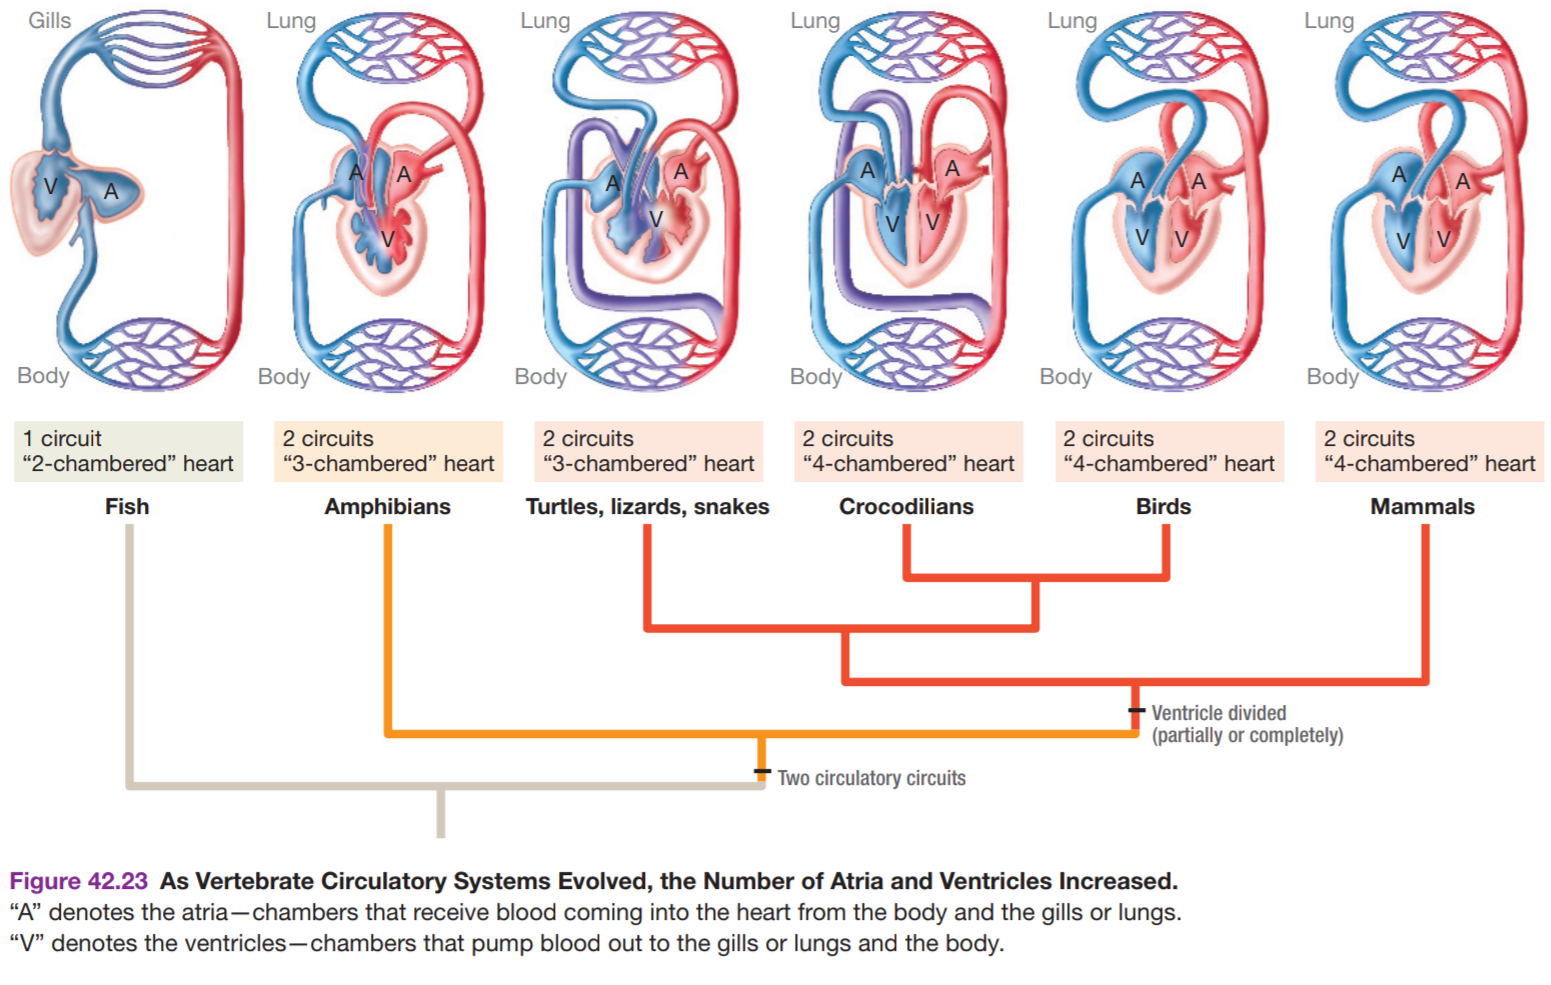
\includegraphics[scale=0.4]{images/hrt.png}    
        \end{center}
        \vspace{-20pt}
        \item \textbf{Venae cavae}: two large veins, called the inferior
        (lower) and superior (upper) venae cavae. Blood low in oxygen returns to the heart via these veins.
        \begin{center}
            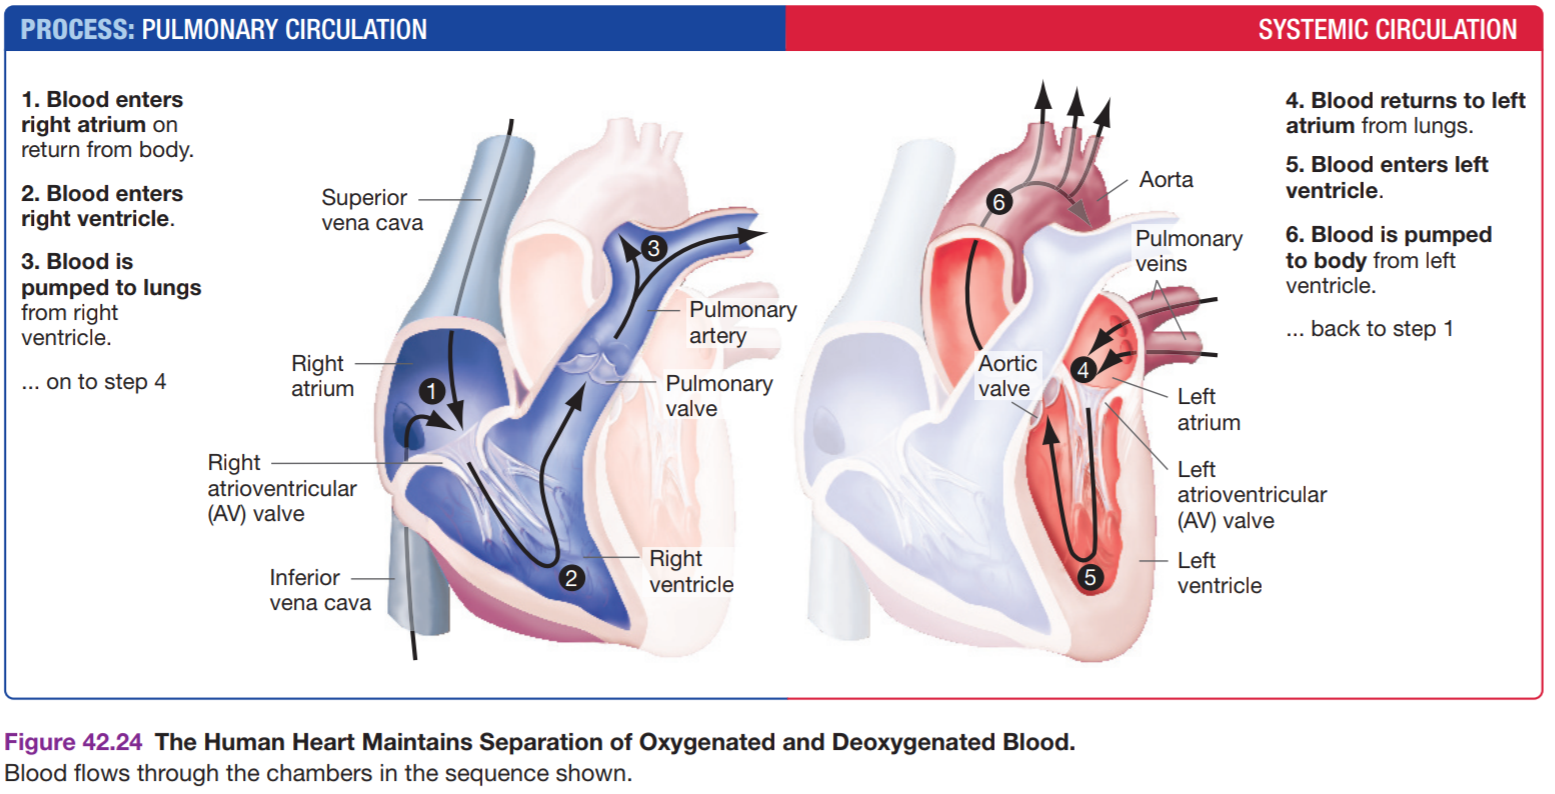
\includegraphics[scale=0.4]{images/hrt2.png}    
        \end{center}
        \vspace{-20pt}
        \item \textbf{Heart murmur}: backflow that reduces the heart's efficiency.
        \item \textbf{Pacemaker cells}: initiate contraction in the vertebrate heart.
        \item \textbf{Sinoatrial (SA) node}: region of the right atrium.
        \item \textbf{Intercalated discs}: connects cardiac muscle cells by joining end to end with other branching cardiac muscle cells.
        \item \textbf{Electrocardiogram}
        \begin{center}
            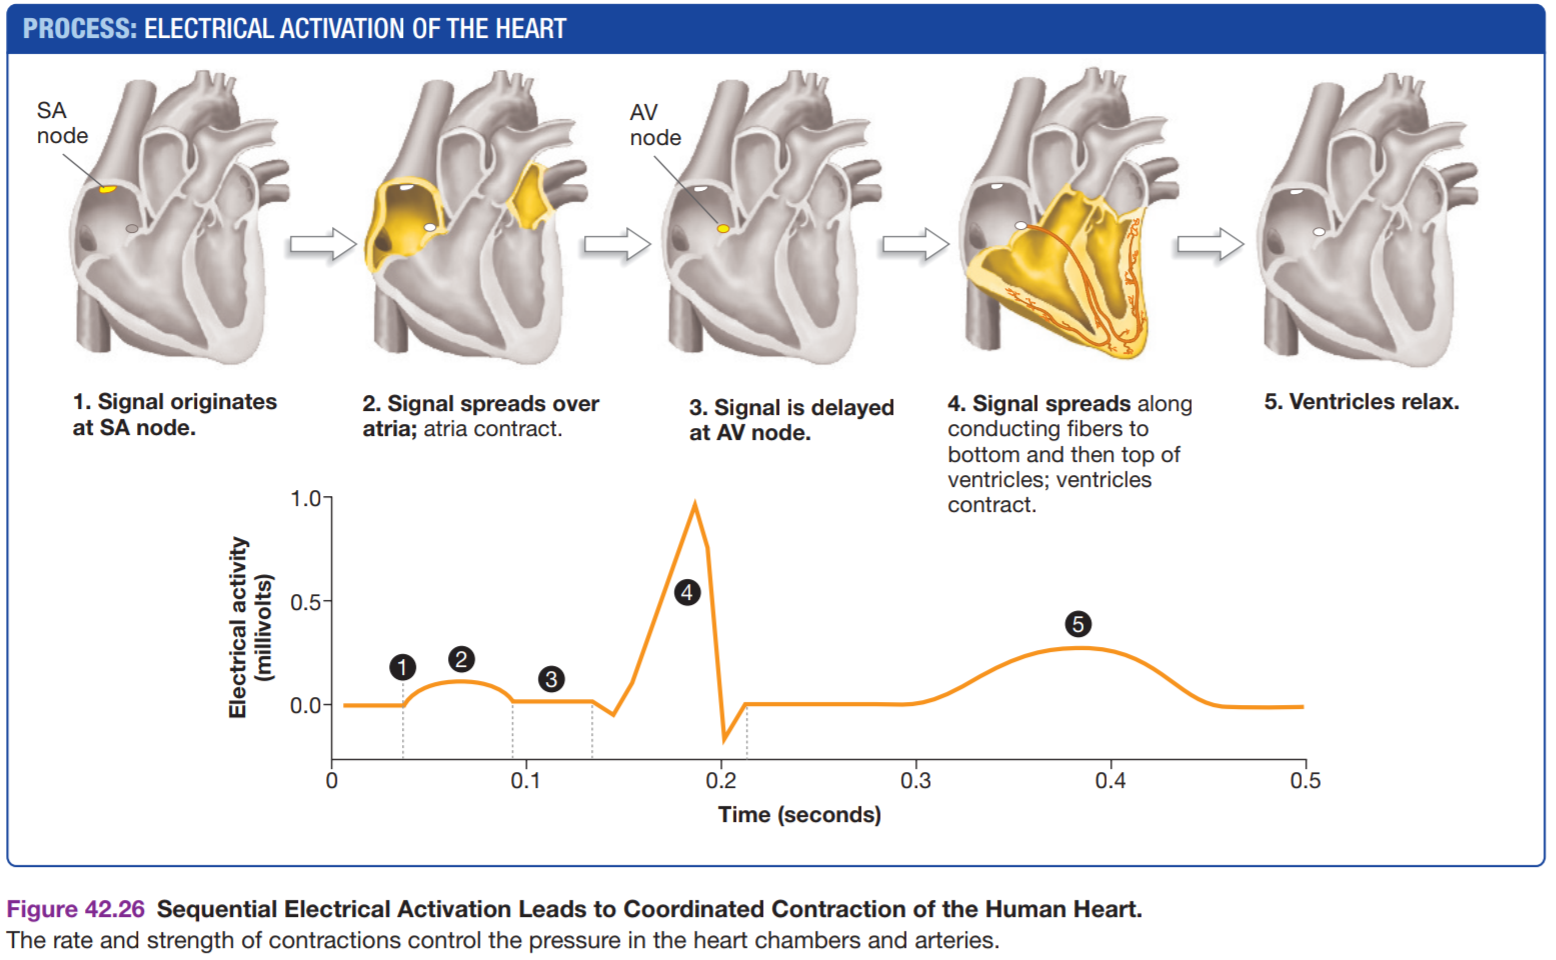
\includegraphics[scale=0.4]{images/ekg.png}    
        \end{center}
        \vspace{-18pt}
        \item \textbf{Systole}: the contraction phases of the atria.
        \item \textbf{Diastole}: the reaction phases of the atria.
        \item \textbf{Cardiac cycle}: consists of one
        diastole and one systole for both atria and ventricles.
        \item \textbf{Systolic blood pressure}: blood pressure measured
        in the systemic arterial circulation at the peak of ventricular ejection into the aorta.
        \item \textbf{Diastolic blood pressure}: blood
        pressure measured just before ventricular ejection is called the
        \item \textbf{Hypertension}: people with blood pressures consistently higher than 140/90 mm Hg.
        \item \textbf{Baroreceptors}: pressure-sensing receptors that detect changes in blood pressure.
        \item \textbf{Arteriosclerosis}: a condition where blood vessels harden and lose elasticity.
        \item \textbf{Myocardial infarction}: arteries that deliver blood to the heart muscle become completely blocked, causing heart attack. 
    \end{itemize}
}\end{secbox}

\hypertarget{42.r}{}
\begin{probbox}{\hyperlink{42}{Chapter 42: Review}}{
    \hyperlink{42.1}{The Resipitory and Circulatory System}
    \begin{itemize}
        \item Animal gas exchange involves ventilation, exchange of gases between the environment and the blood, and exchange of gases between blood and tissues. 
        \item Animal circulation involves transportation of gases, nutrients, wastes, and other substances throughout the body.
    \end{itemize}
    \hyperlink{42.2}{Air and Water as Resipitory Media}
    \begin{itemize}
        \item As media for exchanging oxygen and carbon dioxide, air and water are dramatically different. 
        \item Compared with water, air contains much more oxygen and is much less dense and viscous. As a result, terrestrial animals have to process a much smaller volume of air to extract the same amount of O2, and the amount of work required to do so is less than in aquatic animals. 
        \item Both terrestrial and aquatic animals pay a price for exchanging gases: Land-dwellers lose water to evaporation; freshwater animals lose ions and gain excess water; marine animals gain ions and lose water.      
    \end{itemize}
    \hyperlink{42.3}{Organs of Gas Exchange}
    \begin{itemize}
        \item The structure of gills, tracheae, lungs, and other gas exchange organs minimizes the cost of ventilation while maximizing the diffusion rates of O2 and CO2. 
        \item Consistent with predictions made by Fick’s law of diffusion, respiratory epithelia tend to be extremely thin and to be folded to increase surface area. 
        \item In fish gills, countercurrent exchange ensures that the differences in O2 and CO2 partial pressures between water and blood are favorable for gas exchange over the entire length of the ventilatory surface. 
        \item Insect tracheae carry air directly to and from tissues. 
        \item In bird lungs, structural adaptations lead to a high ratio of useful ventilatory space to dead space. 
        \item Breathing rate is regulated to keep the carbon dioxide content of the blood stable during rest and exercise.
    \end{itemize}
    \hyperlink{42.4}{How are Oxygen and Carbon Dioxide Transported in Blood?}
    \begin{itemize}
        \item The tendency of hemoglobin to give up oxygen varies as a function of the PO2 in surrounding tissue in a sigmoidal fashion. As a result, a relatively small change in tissue PO2 causes a large change in the amount of oxygen released from hemoglobin. 
        \item Oxygen binds less tightly to hemoglobin when pH is low. Because CO2 reacts with water to form carbonic acid, the existence of high CO2 partial pressures in exercising muscle tissues lowers their pH and makes oxygen less likely to stay bound to hemoglobin and more likely to be unloaded into tissues. 
        \item The CO2 that diffuses into red blood cells from tissues is rapidly converted to carbonic acid by the enzyme carbonic anhydrase. The protons that are released as carbonic acid dissociates bind to deoxygenated hemoglobin. In this way, hemoglobin acts as a buffer that takes protons out of solution and prevents large fluctuations in blood pH.
    \end{itemize}
    \hyperlink{42.5}{Circulation}
    \begin{itemize}
        \item In many animals, blood or hemolymph moves through the body via a circulatory system consisting of a pump (heart) and vessels. 
        \item In open circulatory systems, overall pressure is low and tissues are bathed directly in hemolymph. 
        \item In closed circulatory systems, blood is contained in vessels that form a continuous circuit. Containment of blood allows higher pressures and flow rates, as well as the ability to direct blood flow accurately to tissues that need it the most. 
        \item In organisms with a closed circulatory system, a lymphatic system collects excess fluid that leaks from the capillaries and returns it to the circulation. 
        \item In amphibians and some reptiles, blood from the pulmonary and systemic circuits may be mixed in the single ventricle. 
        \item In mammals and birds, a four-chambered heart pumps blood into two circuits, which separately serve the lungs and the rest of the body. Crocodilians have a similar heart with a bypass vessel that can shunt blood from the pulmonary to the systemic circuit. 
        \item In vertebrates, the cardiac cycle is controlled by electrical signals that originate in the heart itself. 
        \item Heart rate, cardiac output, and constriction of both arterioles and veins are regulated by chemical signals and by electrical signals from the brain. 
        \item Cardiovascular disease is the leading cause of death in humans.
    \end{itemize}
}\end{probbox}
%\endgroup
%  ^^^^^^^^^^^^^^^^^^^^^^^^^^^^^^^^^^   Chapter 42   ^^^^^^^^^^^^^^^^^^^^^^^^^^^^^^^^^^ %  
%%%%%%%%%%%%%%%%%%%%%%%%%%%%%%%%%%%%%%%%%%%%%%%%%%%%%%%%%%%%%%%%%%%%%%%%%%%%%%%%%%%%%%%%%

%%%%%%%%%%%%%%%%%%%%%%%%%%%%%%%%%%%%%%%%%%%%%%%%%%%%%%%%%%%%%%%%%%%%%%%%%%%%%%%%%%%%%%%%%
%  vvvvvvvvvvvvvvvvvvvvvvvvvvvvvvvvvv   Chapter 43   vvvvvvvvvvvvvvvvvvvvvvvvvvvvvvvvvv %
%\begingroup

\clearpage

\renewcommand{\thetitle}{\hypertarget{43}{Nervous System}}
\rfoot{\hyperlink{43}{43 --- \thepage}}
\hypertarget{43}{}
\setcounter{section}{43}

\begin{chapbox}{\hyperlink{home}{Chapter 43:Nervous System}}
    \begin{enumerate}
        \item \hyperlink{43.1}{Principles of Electric Signaling}
        \item \hyperlink{43.2}{Dissecting Action Potential}
        \item \hyperlink{43.3}{The Synapse}
        \item \hyperlink{43.4}{The Vertebrate Nervous System}
        \item [--] \hyperlink{43.r}{Review}
    \end{enumerate}
\end{chapbox}

\hypertarget{43.1}{}
\begin{secbox}{\hyperlink{43}{Principles of Electric Signaling}}{
    \begin{itemize}
        \item \textbf{Nerve net}
        \item \textbf{Central nervous system (CNS)}
        \item \textbf{Sensory neurons}
        \item \textbf{Interneurons}
        \item \textbf{Motor neurons}
        \item \textbf{Nerves}
        \item \textbf{Peripheral nervous system}
        \item \textbf{Reflex}
        \item \textbf{Cell body}
        \item \textbf{Dendrites}
        \item \textbf{Axons}
        \item \textbf{Electrical potential}
        \item \textbf{Membrane Potential}
        \item \textbf{Resting potential}
        \item \textbf{Ion channel}
        \item \textbf{Leak channels}
        \item \textbf{Equilibrium potential}
        \item \textbf{Action potential }
        \item \textbf{Three-Phase Signal}
            \begin{itemize}
                \item \textbf{Depolarization}
                \item \textbf{Repolarization}
                \item \textbf{Hyperpolarization}
            \end{itemize}
        \item \textbf{Excitable membranes}
    \end{itemize}
}\end{secbox}

\hypertarget{43.2}{}
\begin{secbox}{\hyperlink{43}{Dissecting Action Potential}}{
    \begin{itemize}
        \item \textbf{Voltage-gated channels}
        \item \textbf{Voltage clamping}
        \item \textbf{Patch clamping}
        \item \textbf{Neurotoxins}
        \item \textbf{Action potential propagation}
        \item \textbf{Refractory state}
        \item \textbf{Oligodendrocytes}
        \item \textbf{Schwann cells }
        \item \textbf{Glia}
        \item \textbf{Schwann cells }
        \item \textbf{Glia}
        \item \textbf{Myelin sheath}
        \item \textbf{Node of Ranvier}
        \item \textbf{Multiple sclerosis (MS)}
    \end{itemize}
}\end{secbox}

\hypertarget{43.3}{}
\begin{secbox}{\hyperlink{43}{The Synapse}}{
    \begin{itemize}
        \item \textbf{Synapses}
        \item \textbf{Neurotransmitters}
        \item \textbf{Synaptic cleft}
        \item \textbf{Synaptic vesicles}
        \item \textbf{Presynaptic neuron}
        \item \textbf{Postsynaptic cell}
        \item \textbf{Ligand-gated channels}
        \item \textbf{Second messengers}
        \item \textbf{Excitatory postsynaptic potentials (EPSPs)}
        \item \textbf{Inhibitory postsynaptic potentials (IPSPs)}
        \item \textbf{Summation}
        \item \textbf{Axon hillock}
    \end{itemize}
}\end{secbox}

\hypertarget{43.4}{}
\begin{secbox}{\hyperlink{43}{The Vertebrate Nervous System}}{
    \begin{itemize}
        \item \textbf{Afferent division }
        \item \textbf{Efferent division}
        \item \textbf{Somatic nervous system}
        \item \textbf{Autonomic nervous system}
        \item \textbf{Parasympathetic nervous system}
        \item \textbf{Sympathetic nervous system}
        \item \textbf{Enteric nervous system}
        \item \textbf{General Anatomy of the Human Brain }
            \begin{itemize}
                \item \textbf{Cerebrum}
                \item \textbf{Cerebellum}
                \item \textbf{Diencephalon}
                \item \textbf{Brain stem}
                \item \textbf{Frontal lobe}
                \item \textbf{Parietal lobe}
                \item \textbf{Occipital lobe}
                \item \textbf{Temporal lobe}
                \item \textbf{Corpus callosum}
                \item \textbf{Hippocampus}
            \end{itemize}
        \item \textbf{Optogenetics}
        \item \textbf{Synaptic plasticity}
        \item \textbf{Neurogenesis}
    \end{itemize}
}\end{secbox}

\hypertarget{43.r}{}
\begin{probbox}{\hyperlink{43}{Chapter 43: Review}}{
    \hyperlink{43.1}{Principles of Electric Signaling}
    \begin{itemize}
        \item Most neurons have a cell body, multiple short dendrites that receive signals from other cells, and a single axon that transmits electrical signals to other neurons or to effector cells in glands or muscles. 
        \item Studies of the squid giant axon established that neurons have a resting potential maintained by the sodium–potassium pump and potassium leak channels. When Na+/K+-ATPase hydrolyzes ATP, it transports 3 Na+ out of the cell and 2 K+ in.
    \end{itemize}
    \hyperlink{43.2}{Dissecting Action Potential}
    \begin{itemize}
        \item Most neurons have a cell body, multiple short dendrites that receive signals from other cells, and a single axon that transmits electrical signals to other neurons or to effector cells in glands or muscles. 
        \item Studies of the squid giant axon established that neurons have a resting potential maintained by the sodium–potassium pump and potassium leak channels. When Na+/K+-ATPase hydrolyzes ATP, it transports 3 Na+ out of the cell and 2 K+ in.     
    \end{itemize}
    \hyperlink{43.3}{The Synapse}
    \begin{itemize}
        \item Most neurons have a cell body, multiple short dendrites that receive signals from other cells, and a single axon that transmits electrical signals to other neurons or to effector cells in glands or muscles. 
        \item Studies of the squid giant axon established that neurons have a resting potential maintained by the sodium–potassium pump and potassium leak channels. When Na+/K+-ATPase hydrolyzes ATP, it transports 3 Na+ out of the cell and 2 K+ in.
    \end{itemize}
    \hyperlink{43.4}{The Vertebrate Nervous System}
    \begin{itemize}
        \item Most neurons have a cell body, multiple short dendrites that receive signals from other cells, and a single axon that transmits electrical signals to other neurons or to effector cells in glands or muscles. 
        \item Studies of the squid giant axon established that neurons have a resting potential maintained by the sodium–potassium pump and potassium leak channels. When Na+/K+-ATPase hydrolyzes ATP, it transports 3 Na+ out of the cell and 2 K+ in.
    \end{itemize}
}\end{probbox}
%\endgroup
%  ^^^^^^^^^^^^^^^^^^^^^^^^^^^^^^^^^^   Chapter 43   ^^^^^^^^^^^^^^^^^^^^^^^^^^^^^^^^^^ %  
%%%%%%%%%%%%%%%%%%%%%%%%%%%%%%%%%%%%%%%%%%%%%%%%%%%%%%%%%%%%%%%%%%%%%%%%%%%%%%%%%%%%%%%%%

\end{document}